% NOTE: Sciposter is dependent on the following packages: a0size, boxedminipage, color,
% graphics, ifthen, shadow, times
% You need to have these packages installed for for sciposter to run properly

\documentclass[landscape,20pt]{sciposter}

%%% Document Class Options %%%%
%portrait		% The default, orients paper in portrait mode
%landscape 		% Orients paper in landscape mode		
%boxedsections	% The default, makes section titles appear in boxes
%ruledsections	% Makes section titles appear underlined
%plain sections	% Makes section titles appear plain 


\usepackage{epsfig}
\usepackage{amsmath}
\usepackage{amssymb}
\usepackage{multicol}
\usepackage{wallpaper}
\usepackage{rotating}
\usepackage{verbatim}

\newtheorem{Def}{Definition}
%\renewcommand{\titlesize}{\Huge}
%\renewcommand{\authorsize}{\Large}
%\renewcommand{\instsize}{\large}
\renewcommand{\sectionsize}{\Large}
\title{ Evaluation of a Tangible Interface \\for Architectural Daylighting Analysis}

% The author's or authors' names
\author{\ \\ Joshua Nasman and Barbara Cutler}
 
% insert correct institute name
\institute{Department of Computer Science\\
           Rensselaer Polytechnic Institute\\}

\email{\{nasmaj,cutler\}@cs.rpi.edu}  % shows author email address below institute

\noleftlogo
\norightlogo

\setlength{\wpXoffset}{-30in}
\setlength{\wpYoffset}{-32.2in}
%%%%%%%%%%%%%%%%%%%%%%%%%%%%%%%%%%%%%%%%%%%%%%%%%%%%%%%%%%%%%%%%%%%%%%%%%%%%%%%%
\begin{document}
%%%%%%%%%%%%%%%%%%%%%%%%%%%%%%%%%%%%%%%%%%%%%%%%%%%%%%%%%%%%%%%%%%%%%%%%%%%%%%%%


%\CenterWallPaper{2.1}{sun_sky_light}

%The location where the poster is being presented at (appears as footer)
%\conference{Org Name, Conf Title, Dates, City, State or Country}
\conference{ACM SIGGRAPH Symposium on Interactive 3D Graphics and Games}

\maketitle

%%%%%%%%%%%%%%%%
% LEFT IMAGE
%%%%%%%%%%%%%%%%
\vspace{-6.6in}
\begin{minipage}[b]{12.15in}
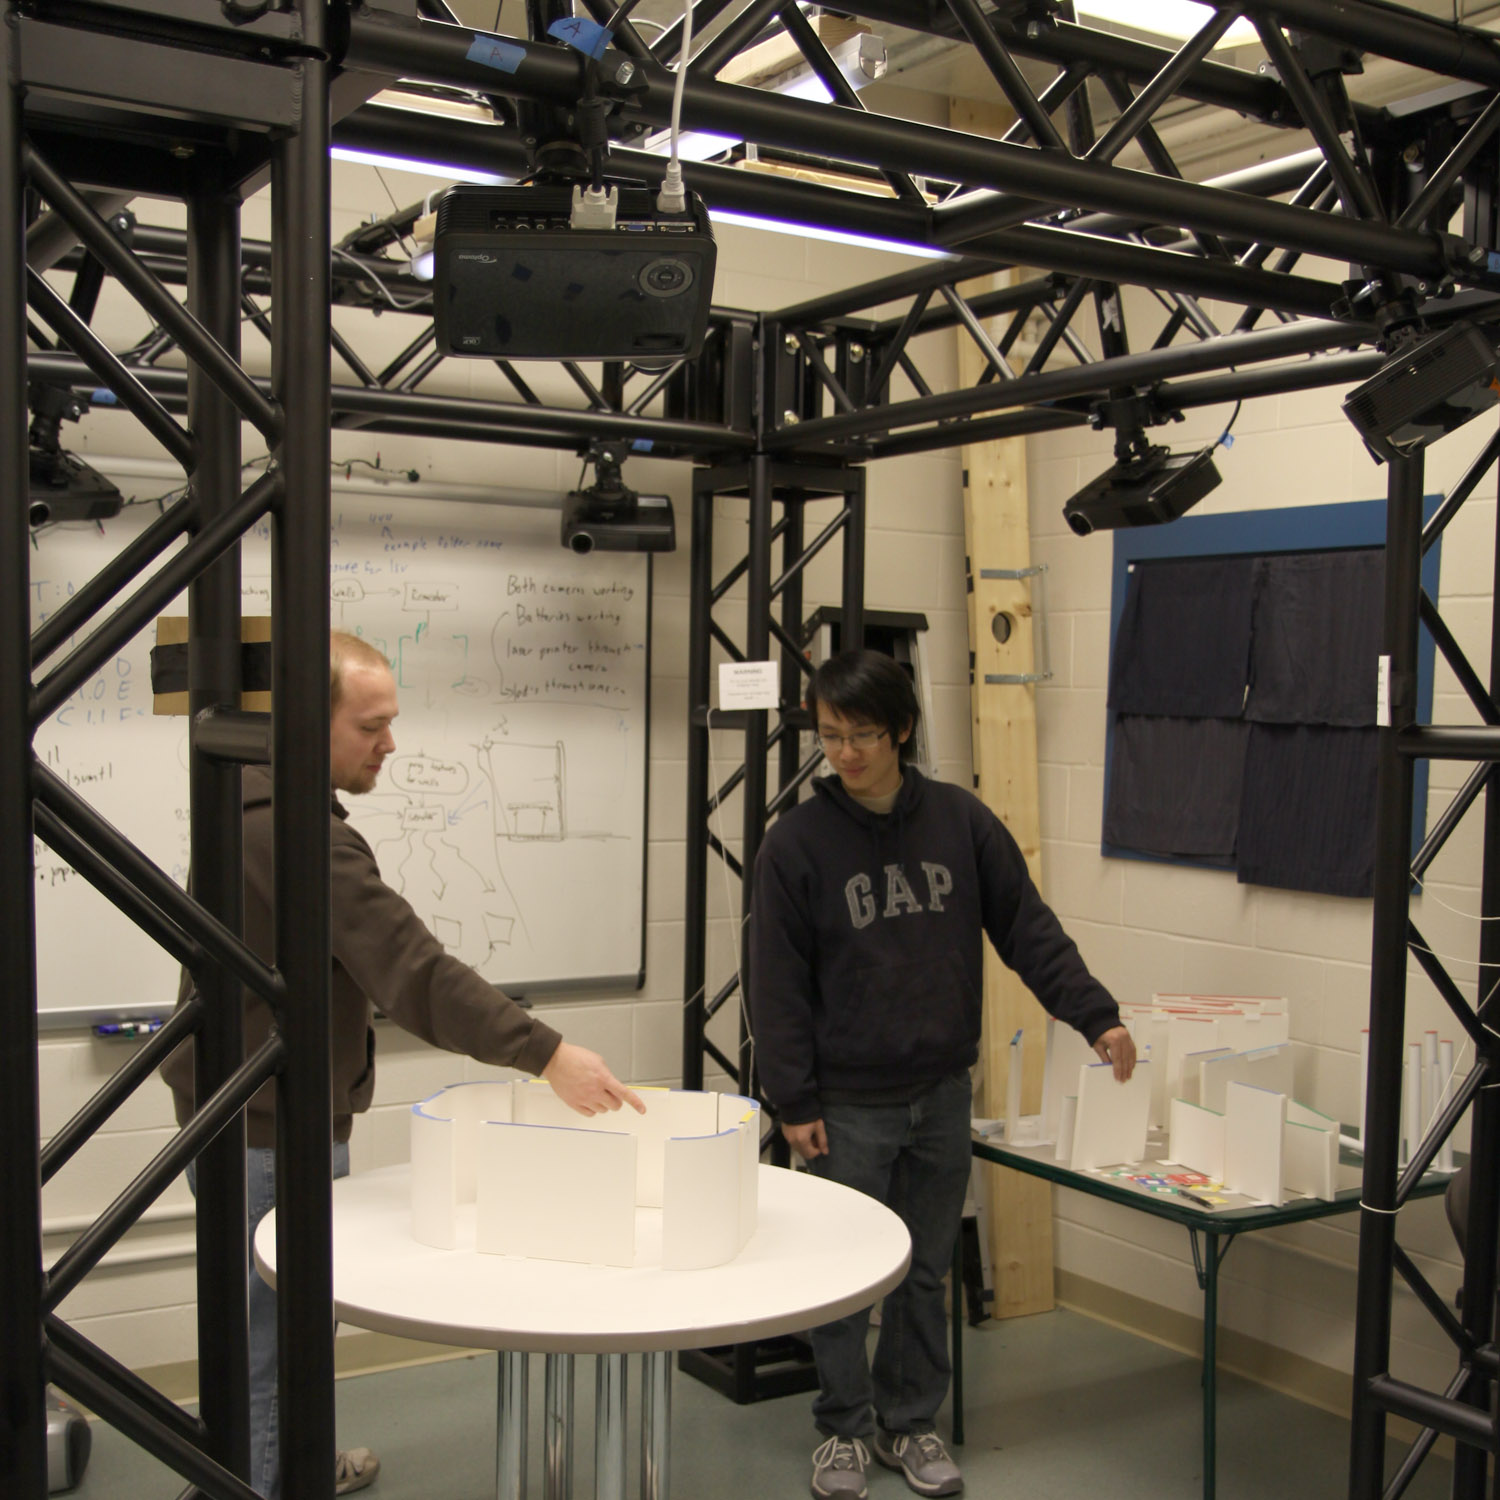
\includegraphics[width=4.in]{../gi2012_userstudy/images/photos/josh_jonathan_new_contraption}
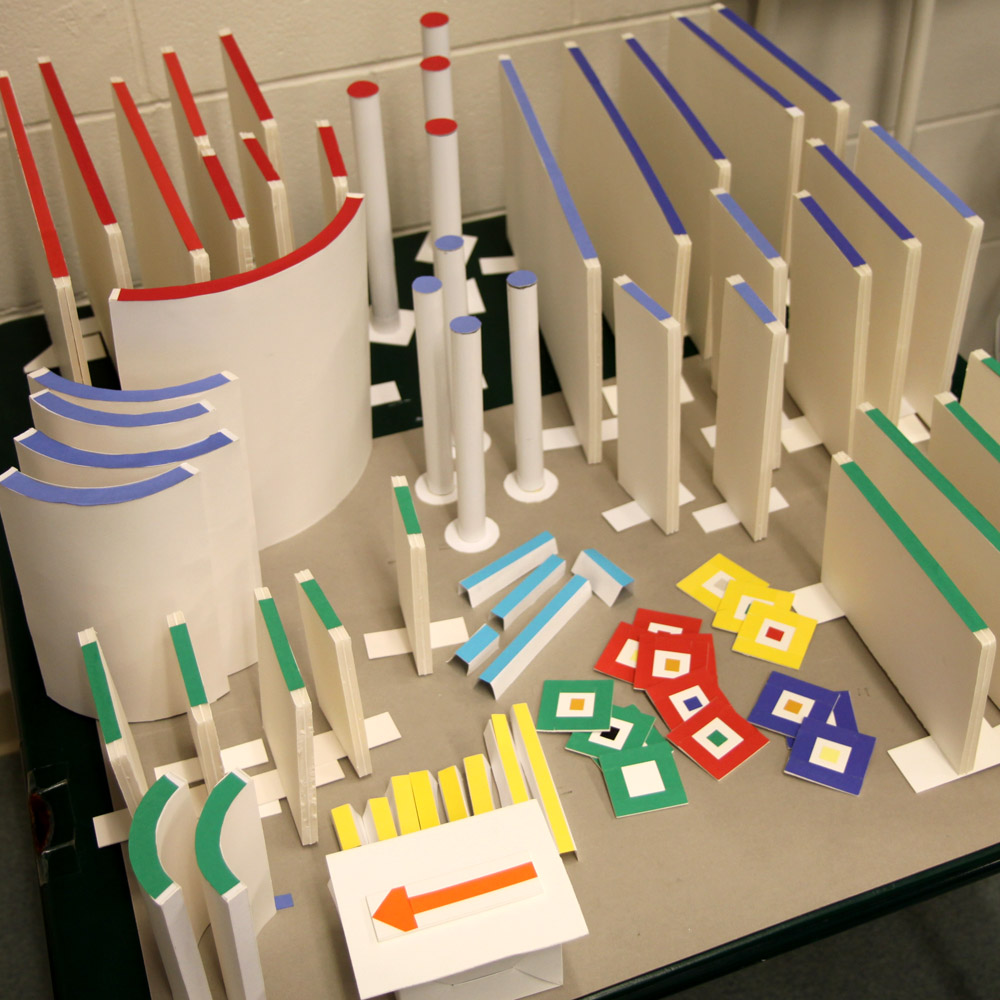
\includegraphics[width=4.in]{../gi2012_userstudy/images/photos/available_wall_pieces}
\begin{minipage}[b]{4in}
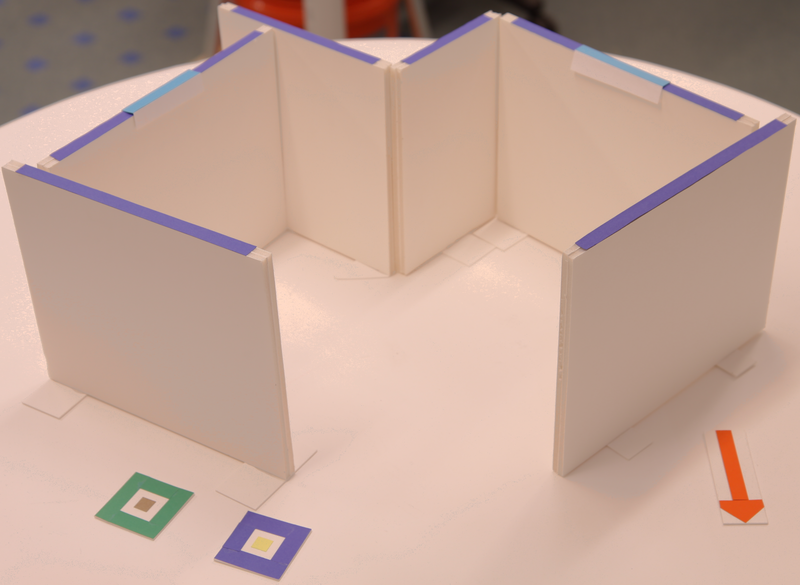
\includegraphics[width=2.85in]{../gi2012_userstudy/images/photos/sample_model}
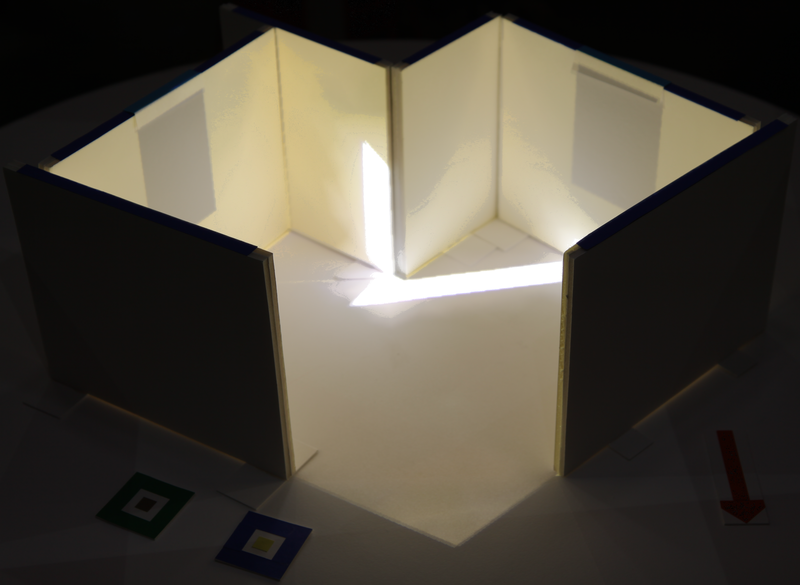
\includegraphics[width=2.85in]{../gi2012_userstudy/images/photos/sample_rendering}
\end{minipage}

\vspace{0.25in}  {\em Our new TUI for architectural daylighting design allows
    multiple users to a) gather around a physical sketching
    environment and select from b) a set of wall primitives and window
    and material markers to c) build a rough sketch of an
    architectural design.  A d) visualization of a daylighting
    simulation is projected onto these surfaces. }
\end{minipage}
\hfill
%
%%%%%%%%%%%%%%%%
% RIGHT IMAGE
%%%%%%%%%%%%%%%%
\begin{minipage}[b]{12.65in}
\resizebox{4.5in}{!}{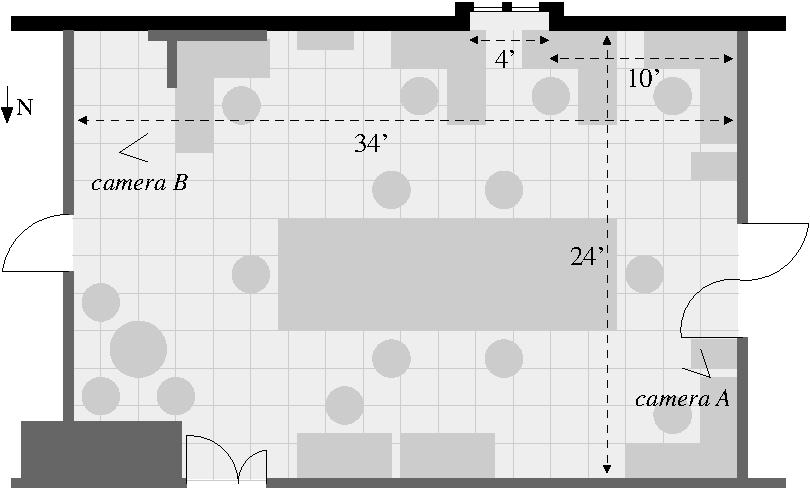
\includegraphics{../gi2012_userstudy/images/lab.pdf}}
\resizebox{4in}{!}{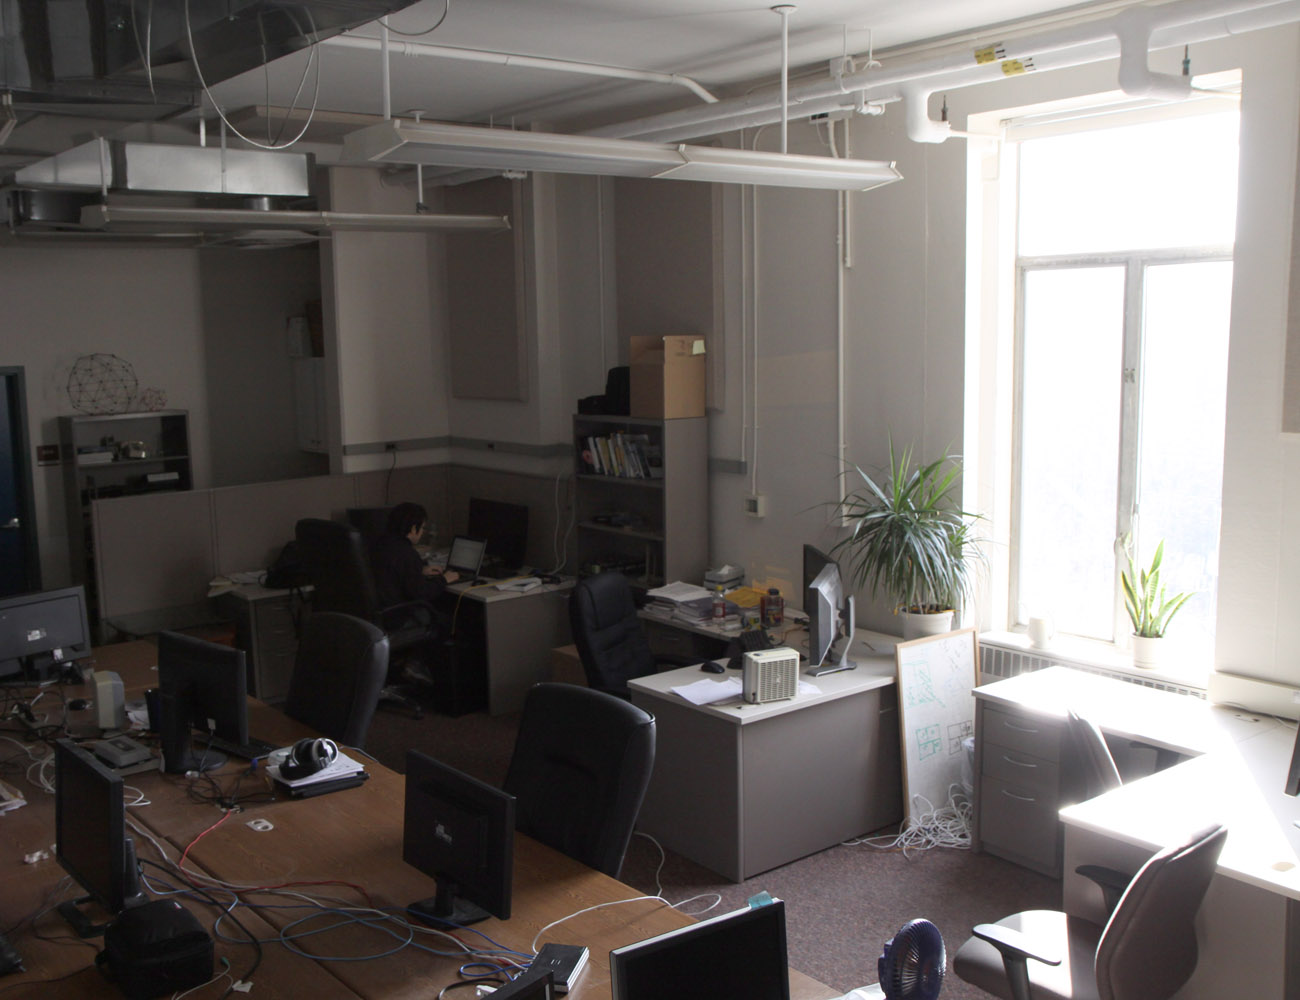
\includegraphics{../gi2012_userstudy/images/photos/camera_angle_2_lights_off.jpg}}
\resizebox{4in}{!}{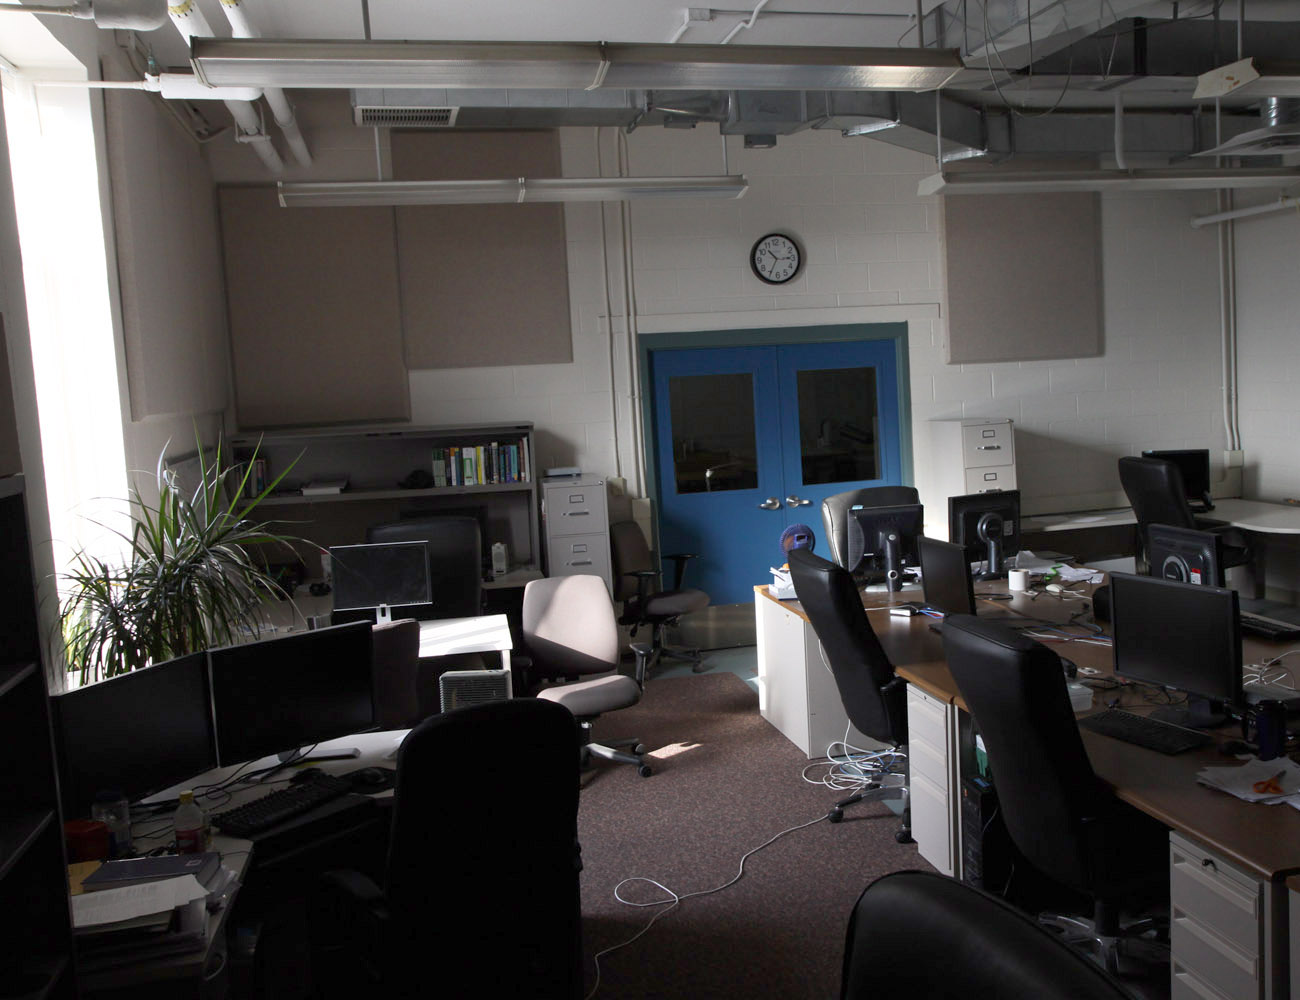
\includegraphics{../gi2012_userstudy/images/photos/camera_angle_3_lights_off.jpg}}
\vspace{-0.5in} \ 
\begin{minipage}{5.5in}\textcolor[rgb]{1,1,1}{\hspace{0.03in} {\bf a)}} \end{minipage}
\begin{minipage}{7in}\textcolor[rgb]{1,1,1}{\hspace{0.03in} {\bf b)}} \end{minipage}
\vspace{0.25in} \\ {\em User study participants visited this simple open office
  environment as a case study for daylighting analysis.  The room
  contains a single, tall and narrow, south-facing window that
  provides direct overly-intense illumination to portions of the room
  while leaving other areas relatively dark.  Thus, occupants of the
  space typically turn on the overhead lights, even on sunny
  afternoons. }
\end{minipage}

\vspace{0.1in}

%%%%%%%%%%%%%%%%%%%%%%%%%%%%%%%%%%%%%%%%%%%%%%%%%%%%%%%%%%%%%%%%%%%%%%%%%%%%%%%%%%%%%%%
%%%%%%%%%%%%%%%%%%%%%%%%%%%%%%%%%%%%%%%%%%%%%%%%%%%%%%%%%%%%%%%%%%%%%%%%%%%%%%%%%%%%%%%

\begin{minipage}[t]{10.5in}
\section*{Overview}
We present a study of a tangible user interface for architectural
design and daylighting analysis.  This tool provides an intuitive way
for architects and future occupants to quickly construct physical
models and then view a simulation of daylighting in the model at
interactive rates.
%
%\fbo{blah sentence}
%User studies are an effective way to obtain both qualitative and
%quantitative feedback for user interfaces.
%
We conducted a user study of both formally-trained architects and
non-architects in a set of analysis and design exercises.
%
This study investigates the effectiveness of this interface as an
educational tool, the precision and accuracy of the constructed
physical models, and the overall effectiveness of the tangible
interface.  The four part study investigates users' intuitions about
daylighting and their interaction with the tool for analysis of an
existing space, for proposing renovations to the space, and for
designing a totally new space with the same architectural program that
better addresses the occupants' needs.  These exercises revealed
misconceptions in many of the participants' intuitions about
daylighting and overall the participants expressed interest in this
simulation tool for daylighting analysis in architectural design.
%
%
\vspace{.3in}
\section*{Contributions}
\begin{itemize}


\item Exploration of participants' fundamental understanding of
  daylighting design, overlighting, underlighting and glare.\vspace{-0.1in}

\item Quantitative analysis of the users' accuracy in using our
  physical sketching system to model a room they had just visited.\vspace{-0.1in}

\item Evaluation of the participants' use of our tool and their
  perception of quantitative and qualitative daylighting from the 
  displayed simulations.\vspace{-0.1in}

\item Demonstration of our tangible interface as a
  creativity-enhancing tool for architectural daylighting design.


\end{itemize}

\vspace{.3in}

\section*{Sketches of a Space with Problematic Lighting}
%\includegraphics[width=0.19\columnwidth]
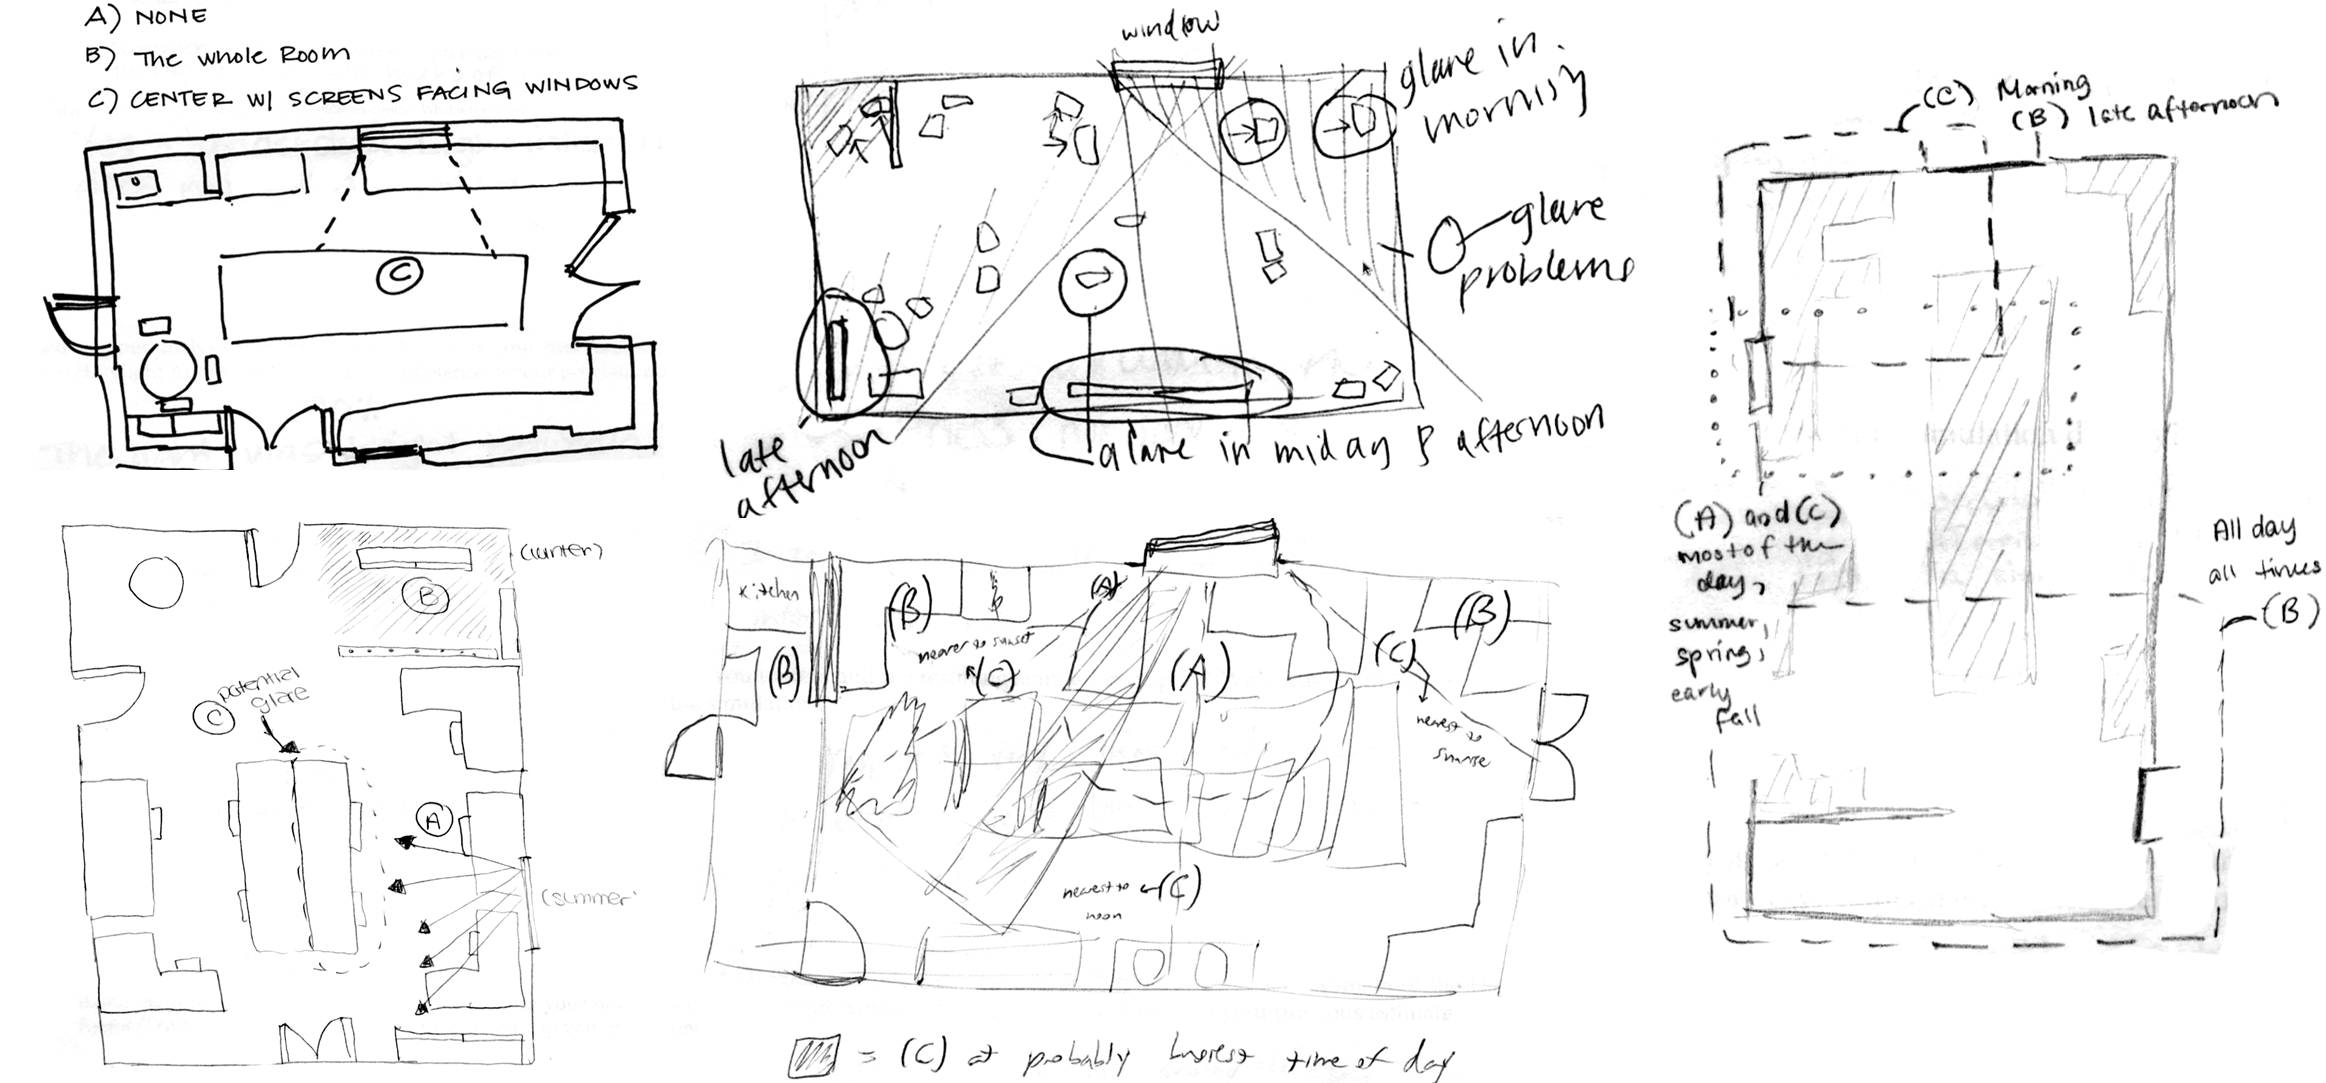
\includegraphics[width=1.00\columnwidth]{../gi2012_userstudy/images/sketches/all_together}%
%
\vspace{-4.8in}
{\bf A4} \hspace{.25\columnwidth}
{\bf A3}
\vspace{4in}
\\
{\bf A5} \hspace{.21\columnwidth}
{\bf N2} \hspace{.45\columnwidth}
{\bf N4}
\vspace{.5in}\\
%
{\em
In Part 1 of the study, participants were asked to sketch the
  lab room and annotate this sketch with their intuition about areas
  with A) too much daylighting, B) too little daylighting, and C)
  potential for glare.  The sketches demonstrate a variety of detail
  and accuracy in the analysis of the dynamic lighting conditions.}

\begin{comment}
\vspace{0.4in}

\resizebox{0.326\columnwidth}{!}{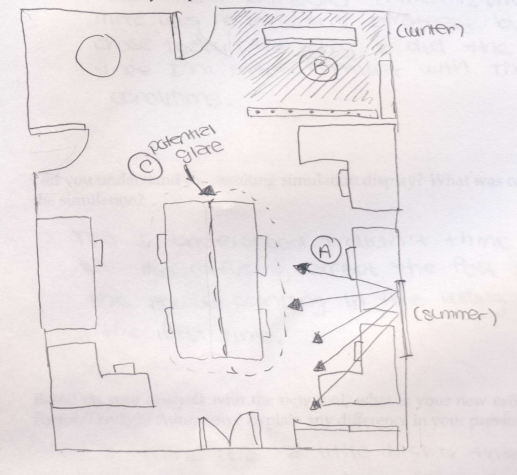
\includegraphics{test}}
\resizebox{0.326\columnwidth}{!}{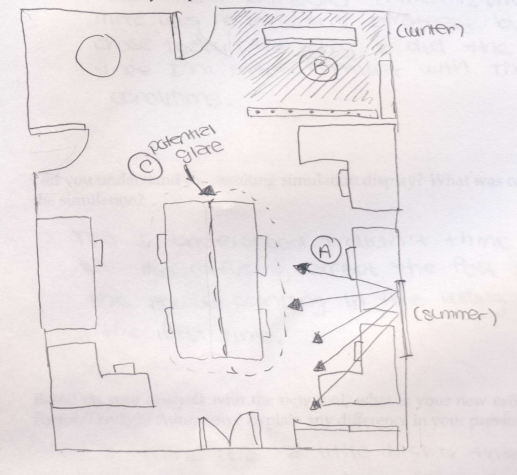
\includegraphics{test}}
\resizebox{0.326\columnwidth}{!}{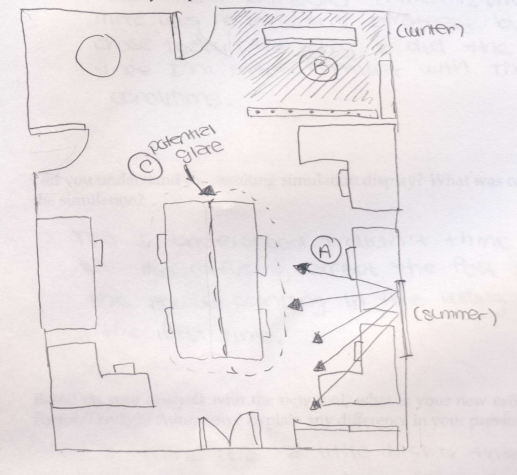
\includegraphics{test}}
\vspace{-0.7in} \ \\
\begin{minipage}{0.326\columnwidth}\textcolor[rgb]{1,1,1}{\hspace{0.05in} {\bf 380 lux}} \end{minipage}
\begin{minipage}{0.326\columnwidth}\textcolor[rgb]{1,1,1}{\hspace{0.05in} {\bf 110 lux}} \end{minipage}
\begin{minipage}{0.326\columnwidth}\textcolor[rgb]{0,0,0}{\hspace{0.05in} {\bf 620 lux}} \end{minipage}
\vspace{-0.1in}\\
\begin{minipage}{0.326\columnwidth}\textcolor[rgb]{0,0,0}{\hspace{1.6in} {\bf 1030 lux}} \end{minipage}
\begin{minipage}{0.326\columnwidth}\textcolor[rgb]{1,1,1}{\hspace{1.6in} {\bf 180 lux}} \end{minipage}
\begin{minipage}{0.326\columnwidth}\textcolor[rgb]{0,0,0}{\hspace{1.6in} {\bf 620 lux}} \end{minipage}
\\
\ \vspace{-0.1in}
\\
{\em On a sunny day with the blinds up (left), parts of
  the conference room table are too bright ($>$ 1000 lux) for
  comfortable reading while other parts are too dark ($<$ 500 lux).
  By closing the blinds we can partially correct the situation by
  removing excess illumination from parts of the table (center).
  Too often in practice, lighting engineers settle for the
  least efficient solution, selecting light
  fixtures for night or when the blinds are fully closed (right).
}
\end{comment}

%%%%%%%%%%%%%%%%%%%%%%%%%%%




\end{minipage}
\hfill
%%%%%%%%%%%%%%%%%%%%%%%%%%%%%%%%%%%%%%%%%%%%%%%%%%%%%%%%%%%%%%%%%%%%%%%%%%%%%%%%%%%%%%%
%
%%%%%%%%%%%%%%%%%%%%%%%%%%%%%%%%%%%%%%%%%%%%%%%%%%%%%%%%%%%%%%%%%%%%%%%%%%%%%%%%%%%%%%%
\begin{minipage}[t]{14in}
\section*{Models of the Example Space}
%
%
  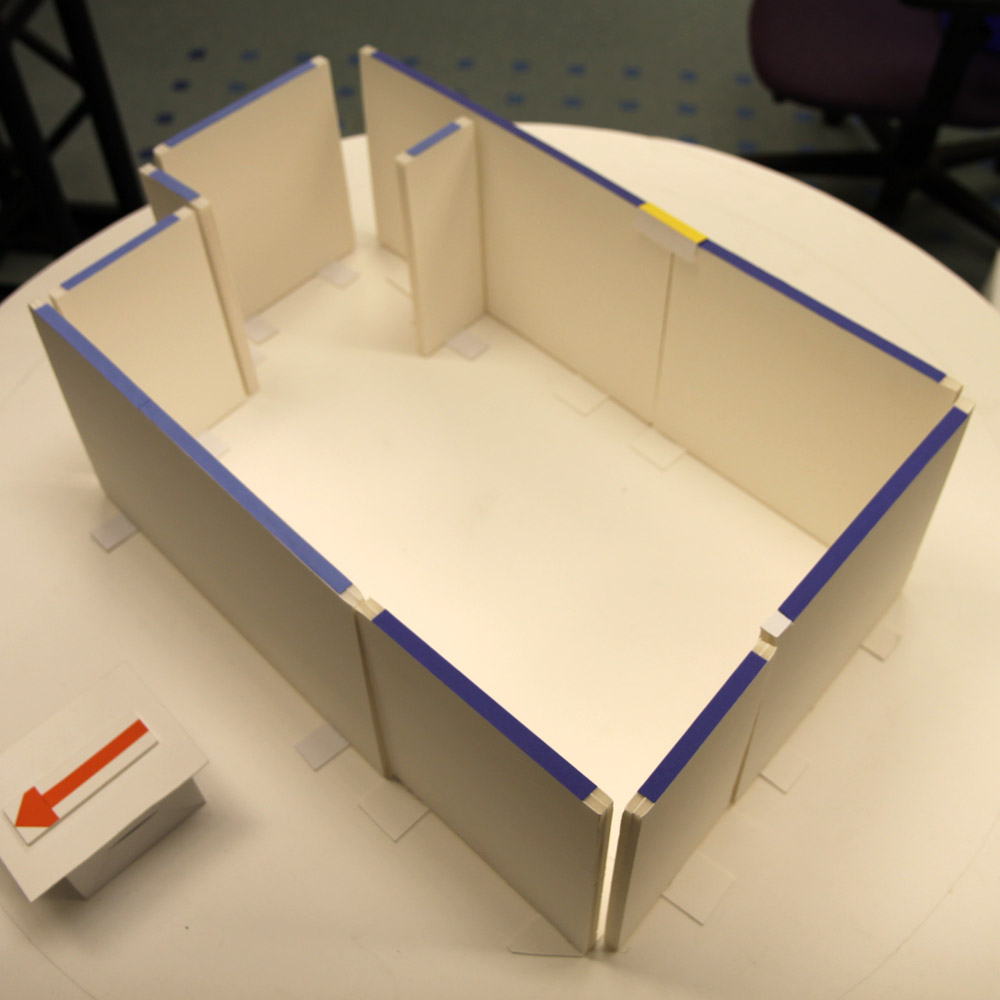
\includegraphics[width=0.19\columnwidth]{../gi2012_userstudy/images/photos/63_original}
%\resizebox{0.7\columnwidth}{!}{ 
  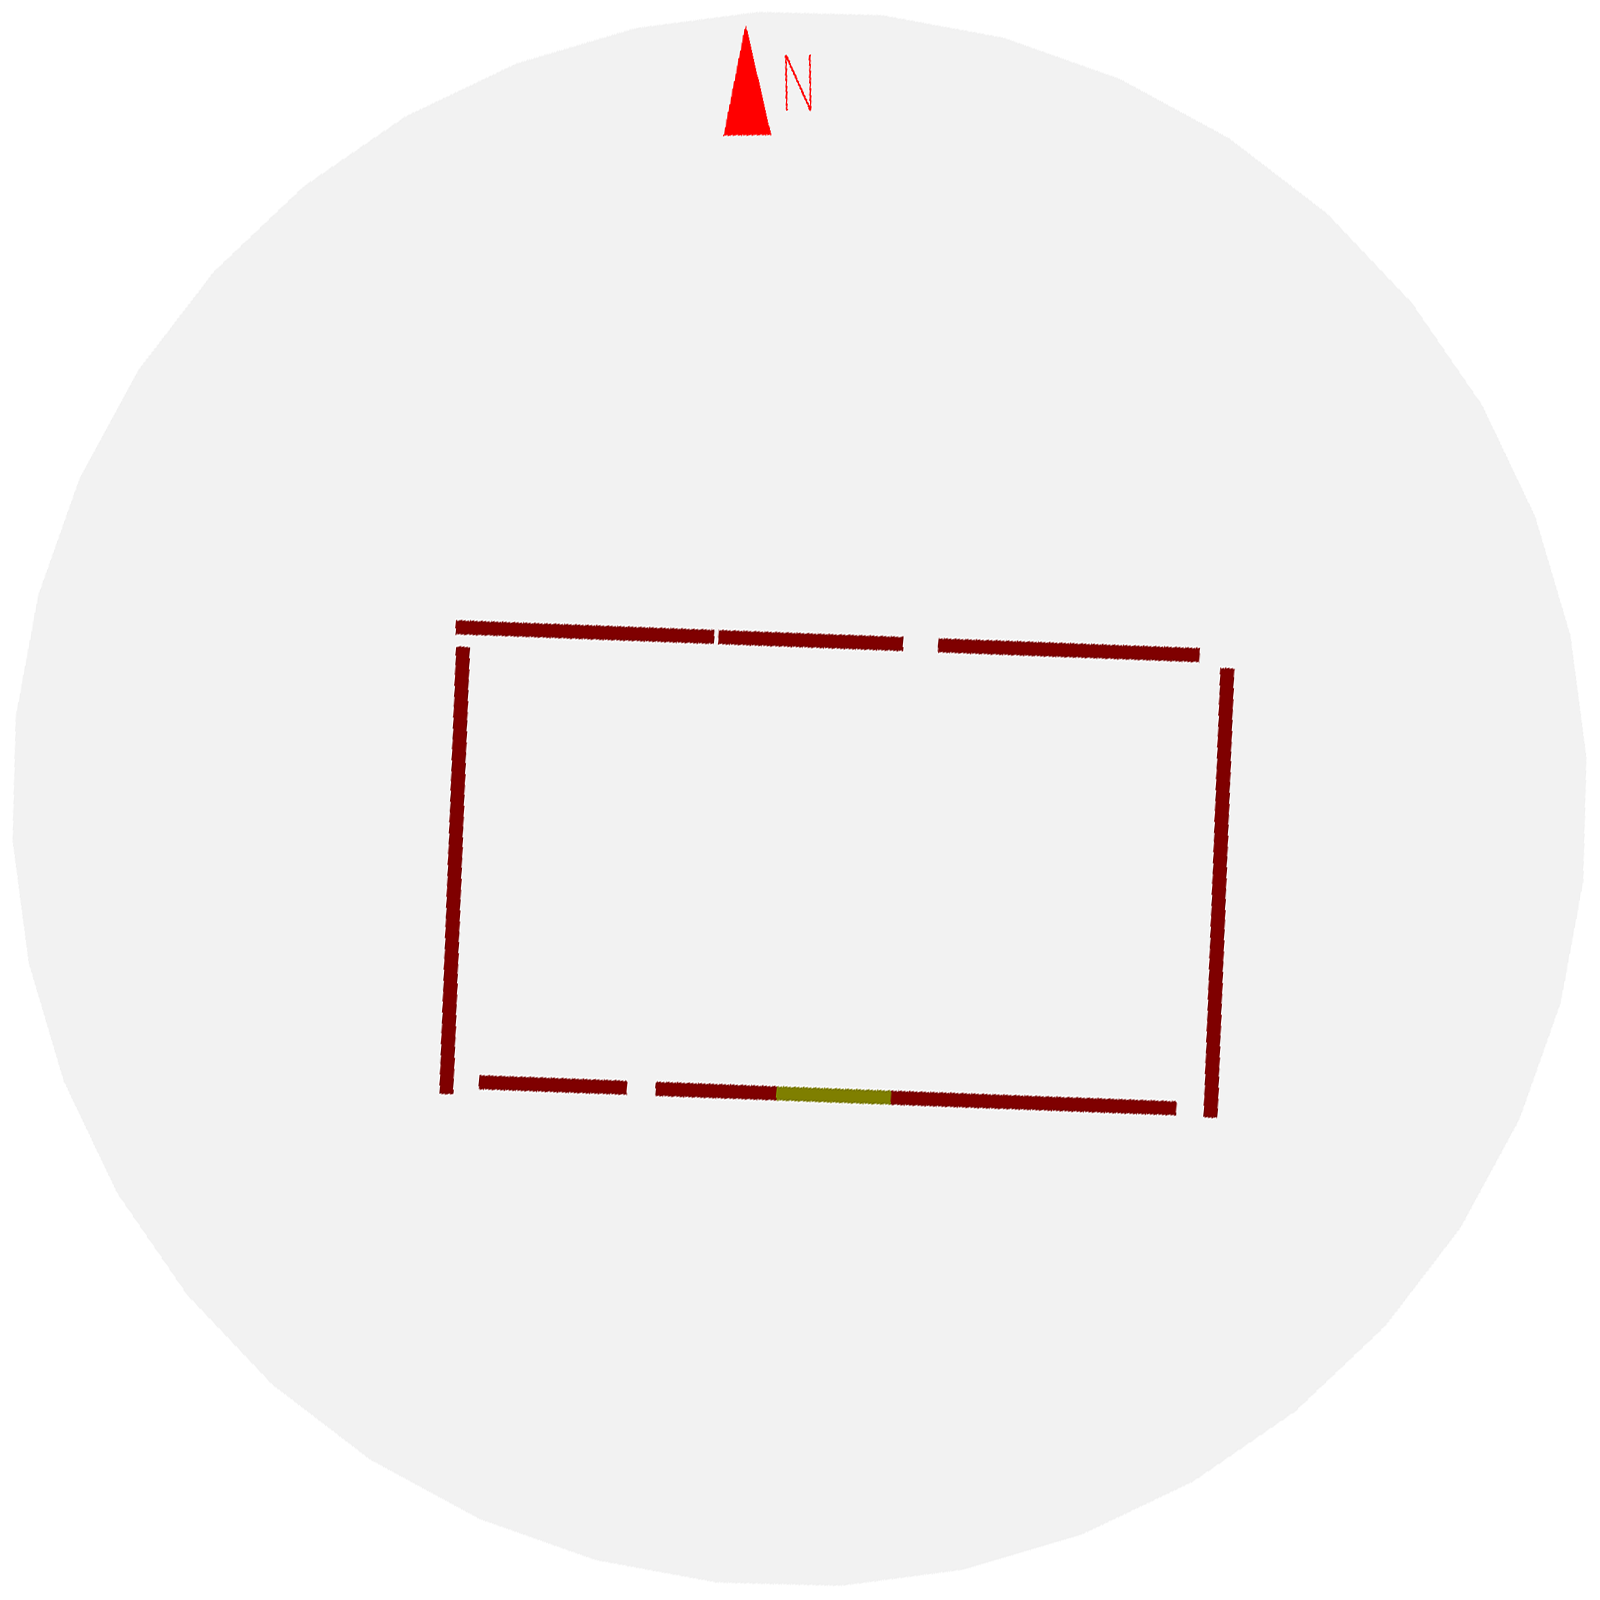
\includegraphics[width=0.19\columnwidth]{../gi2012_userstudy/images/section2/0_2D_walls_rotate} %A1
  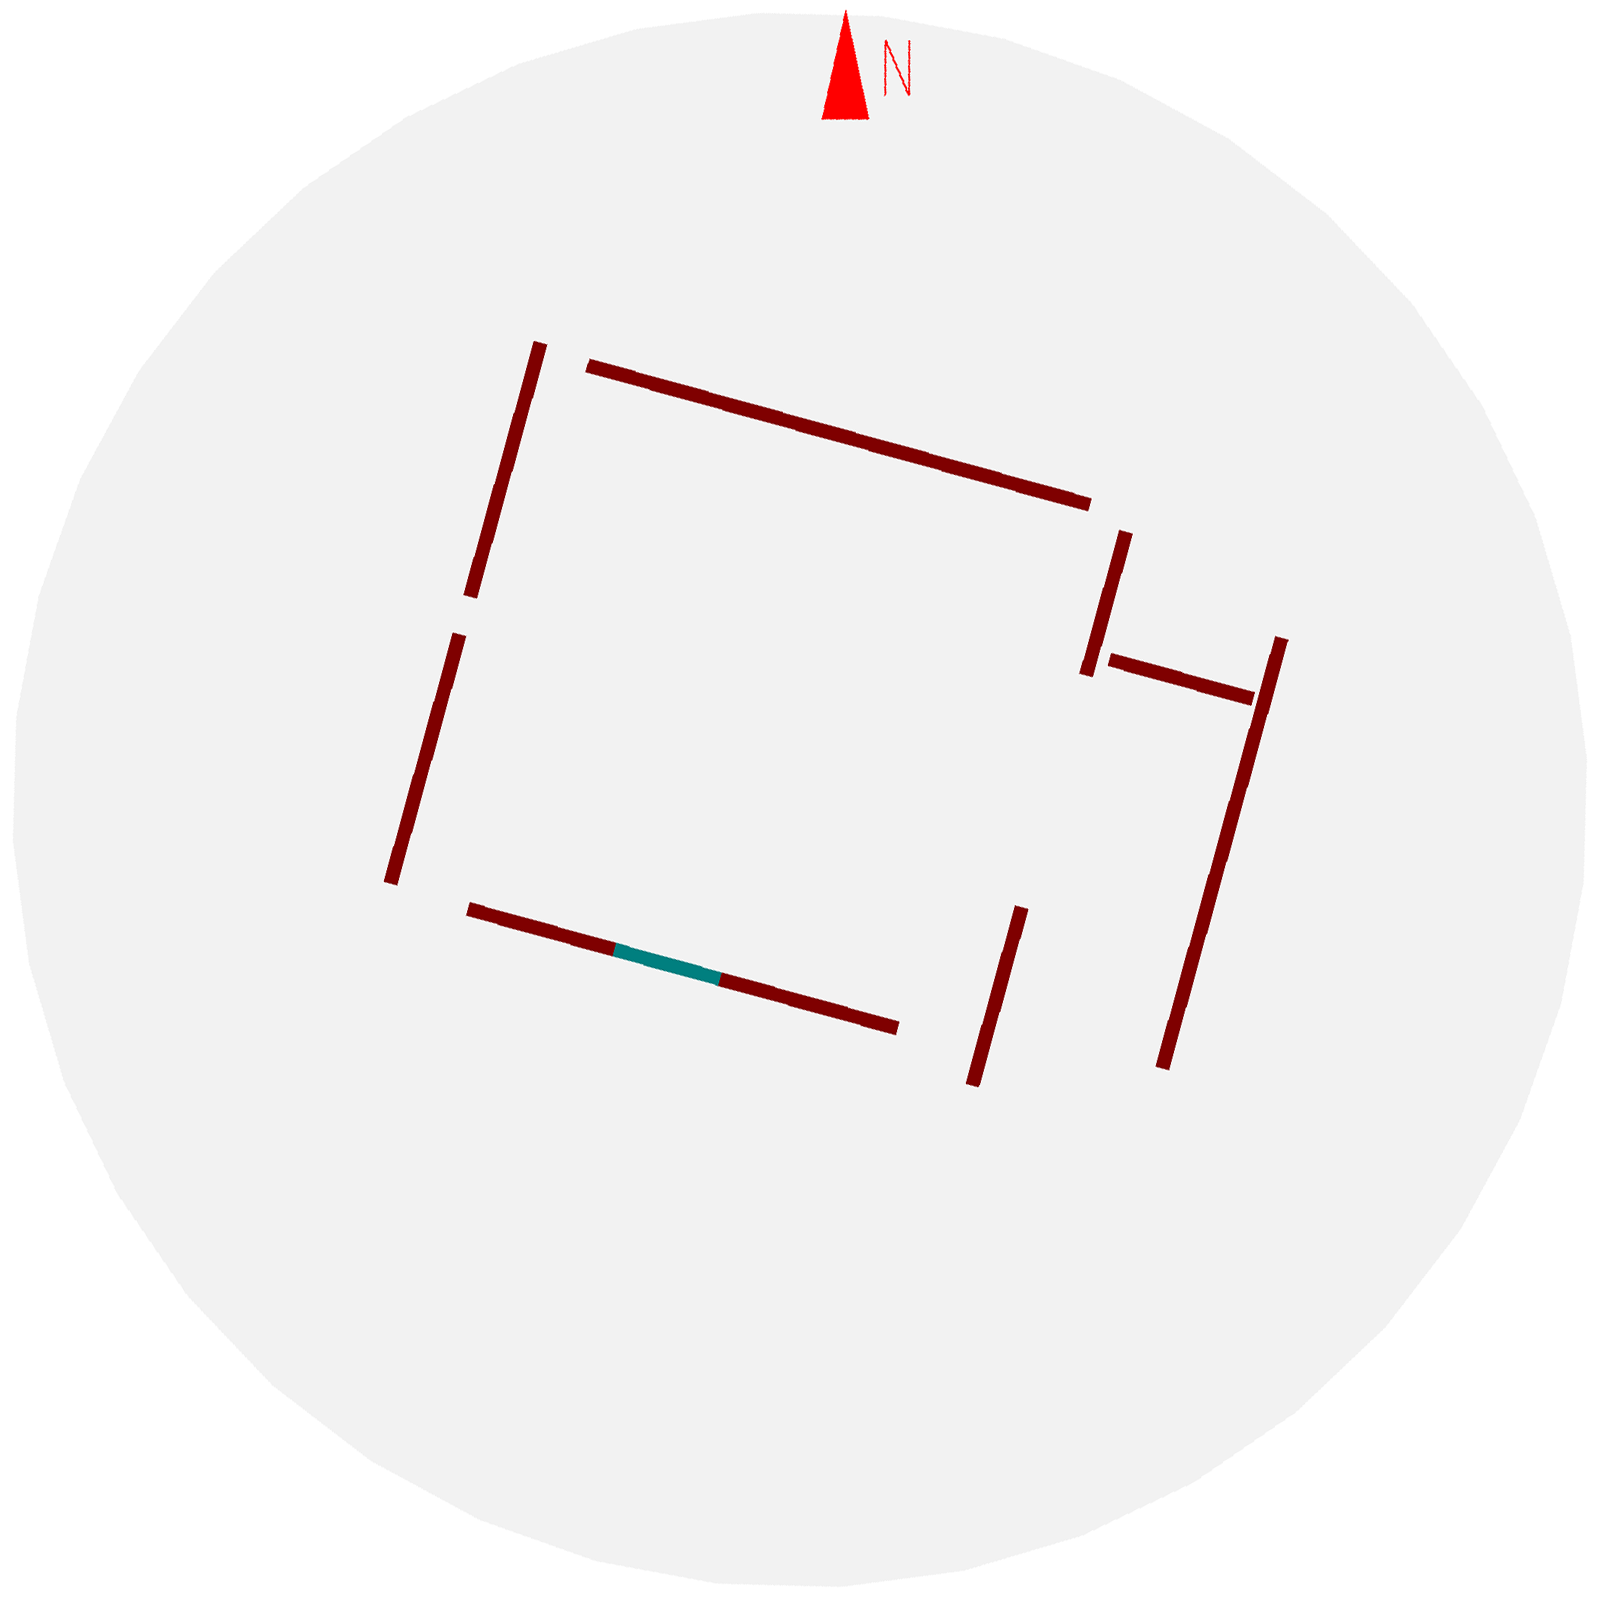
\includegraphics[width=0.19\columnwidth]{../gi2012_userstudy/images/section2/2_2D_walls_rotate} %A2
  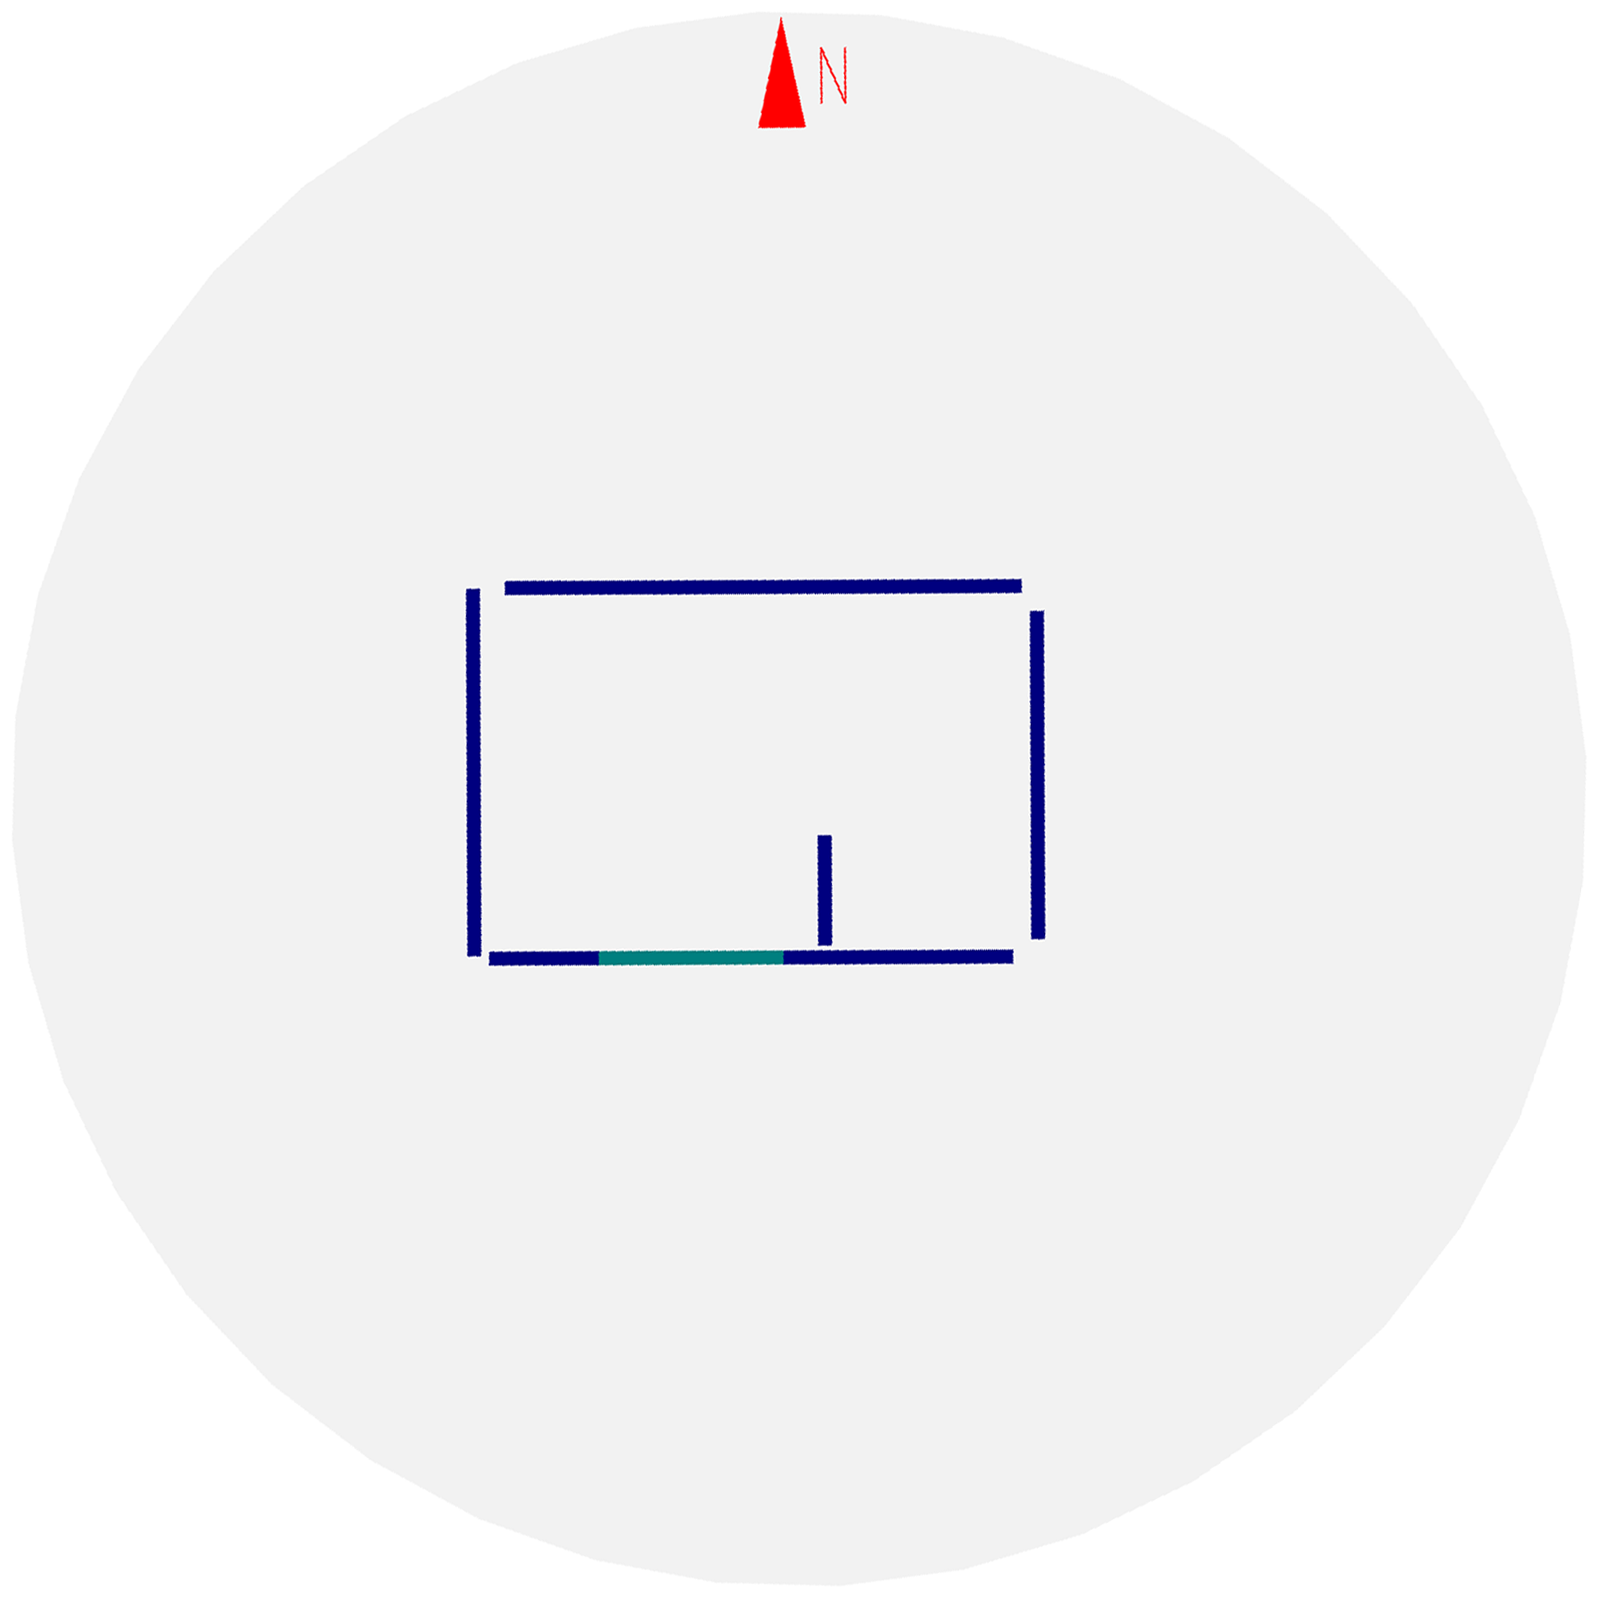
\includegraphics[width=0.19\columnwidth]{../gi2012_userstudy/images/section2/6_2D_walls_rotate}  %A4
  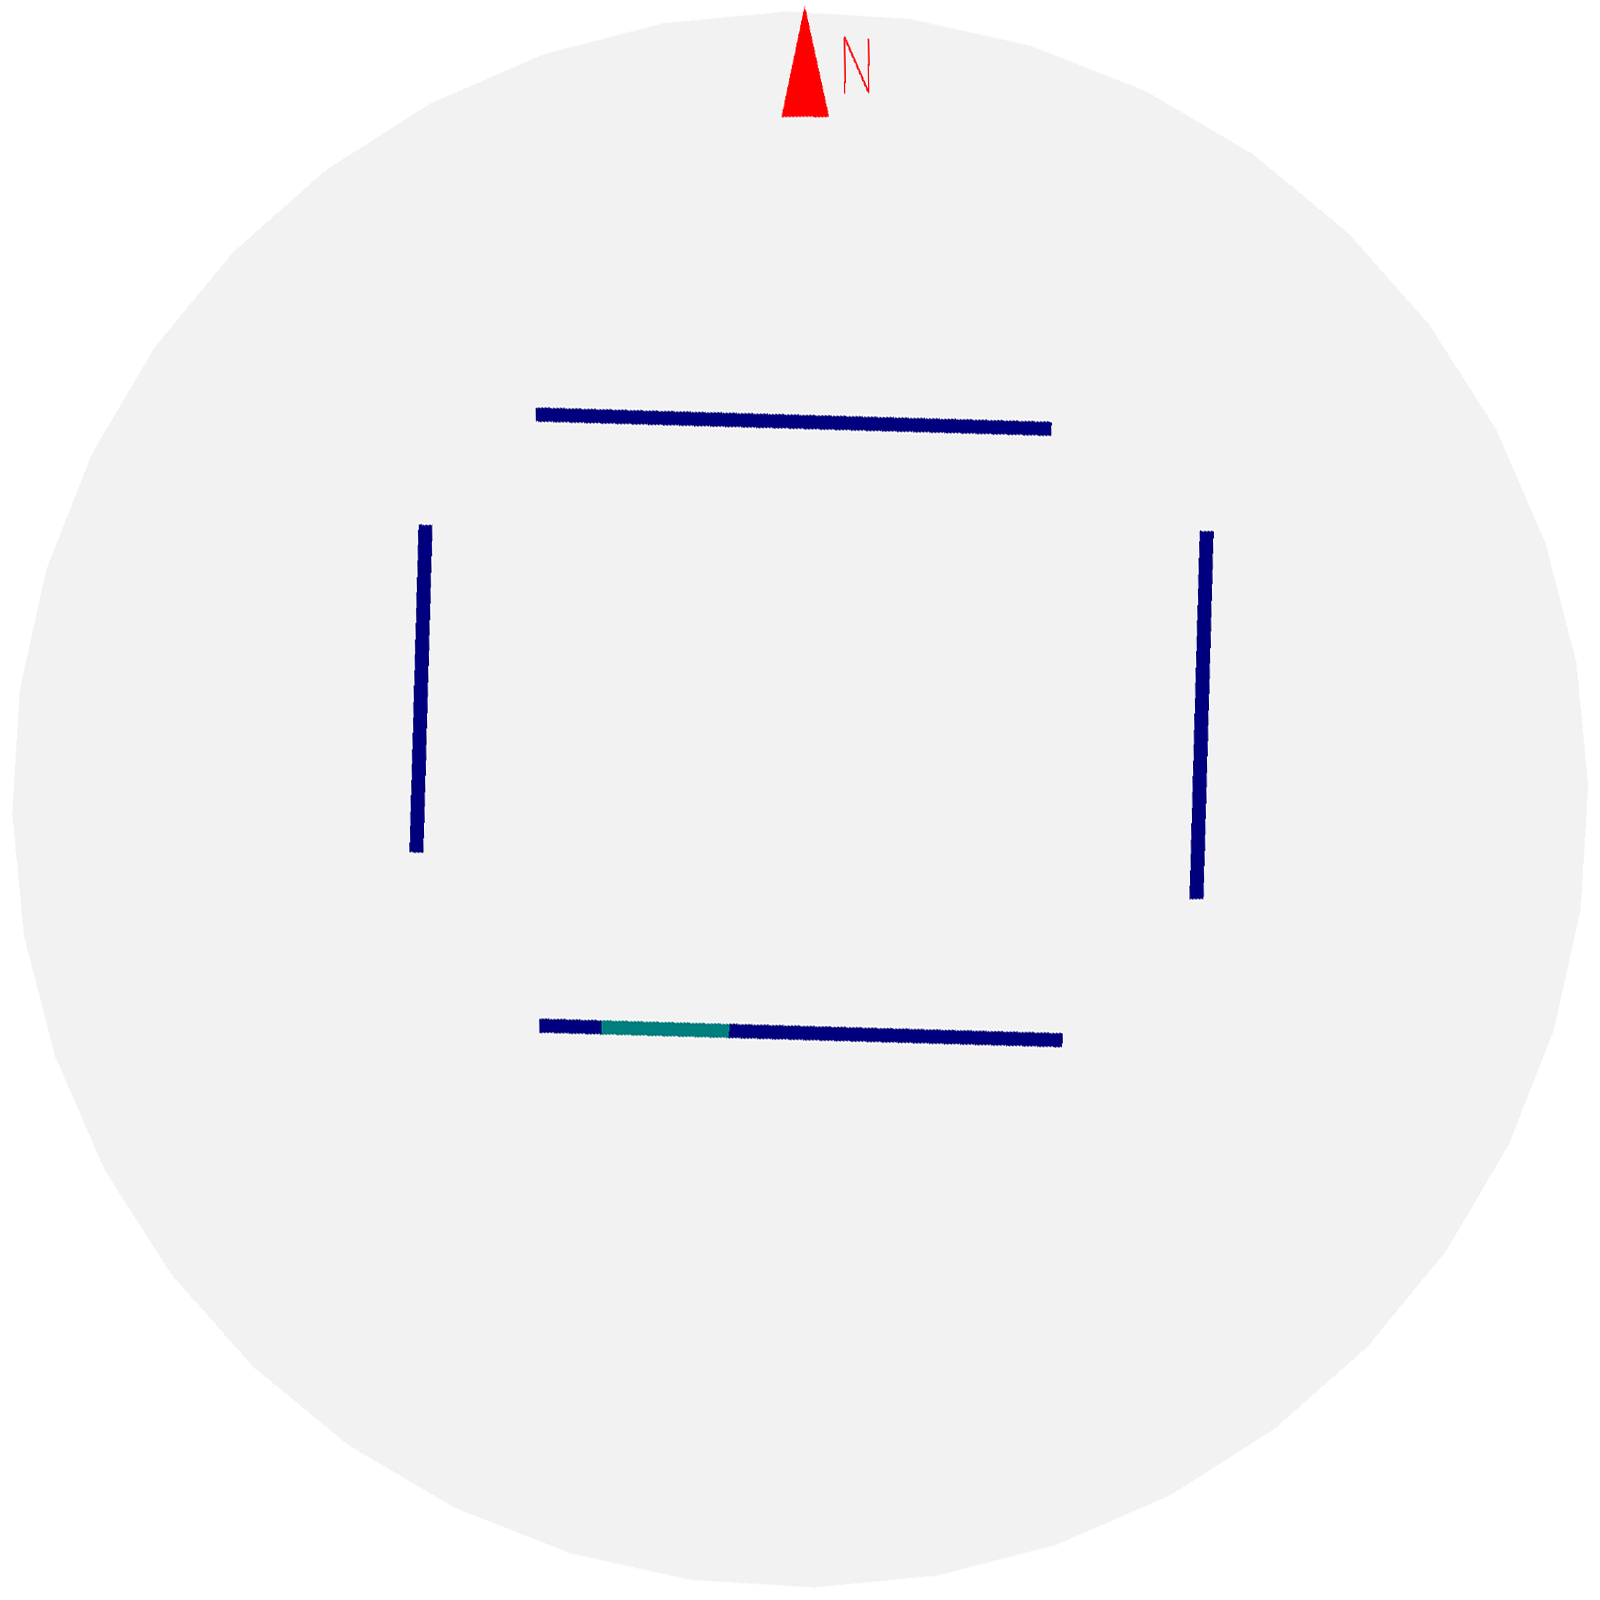
\includegraphics[width=0.19\columnwidth]{../gi2012_userstudy/images/section2/7_2D_walls_rotate}\\ %A5 \\
  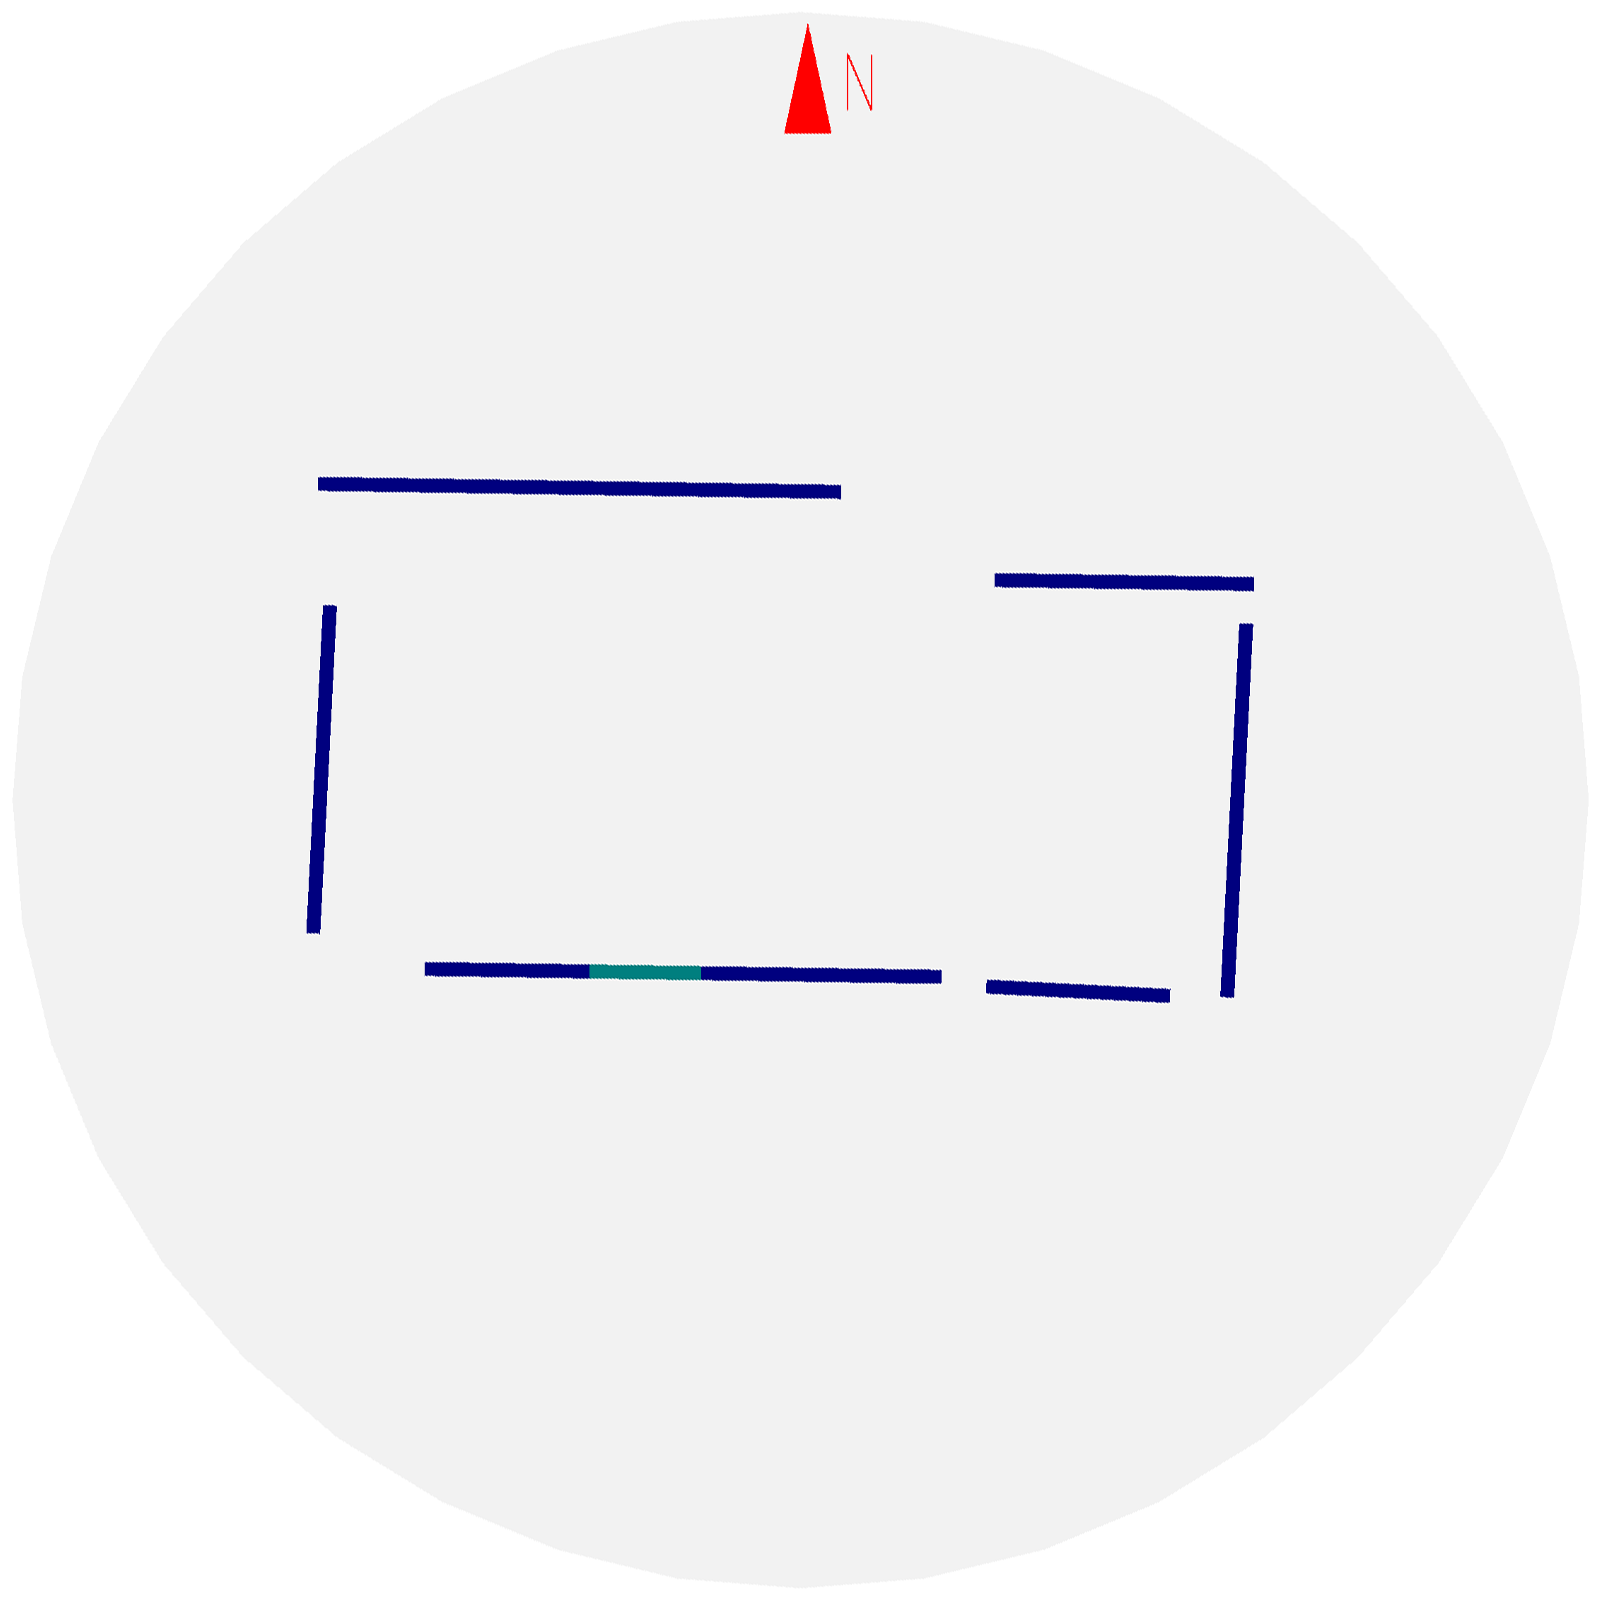
\includegraphics[width=0.19\columnwidth]{../gi2012_userstudy/images/section2/8_2D_walls_rotate} %A6
  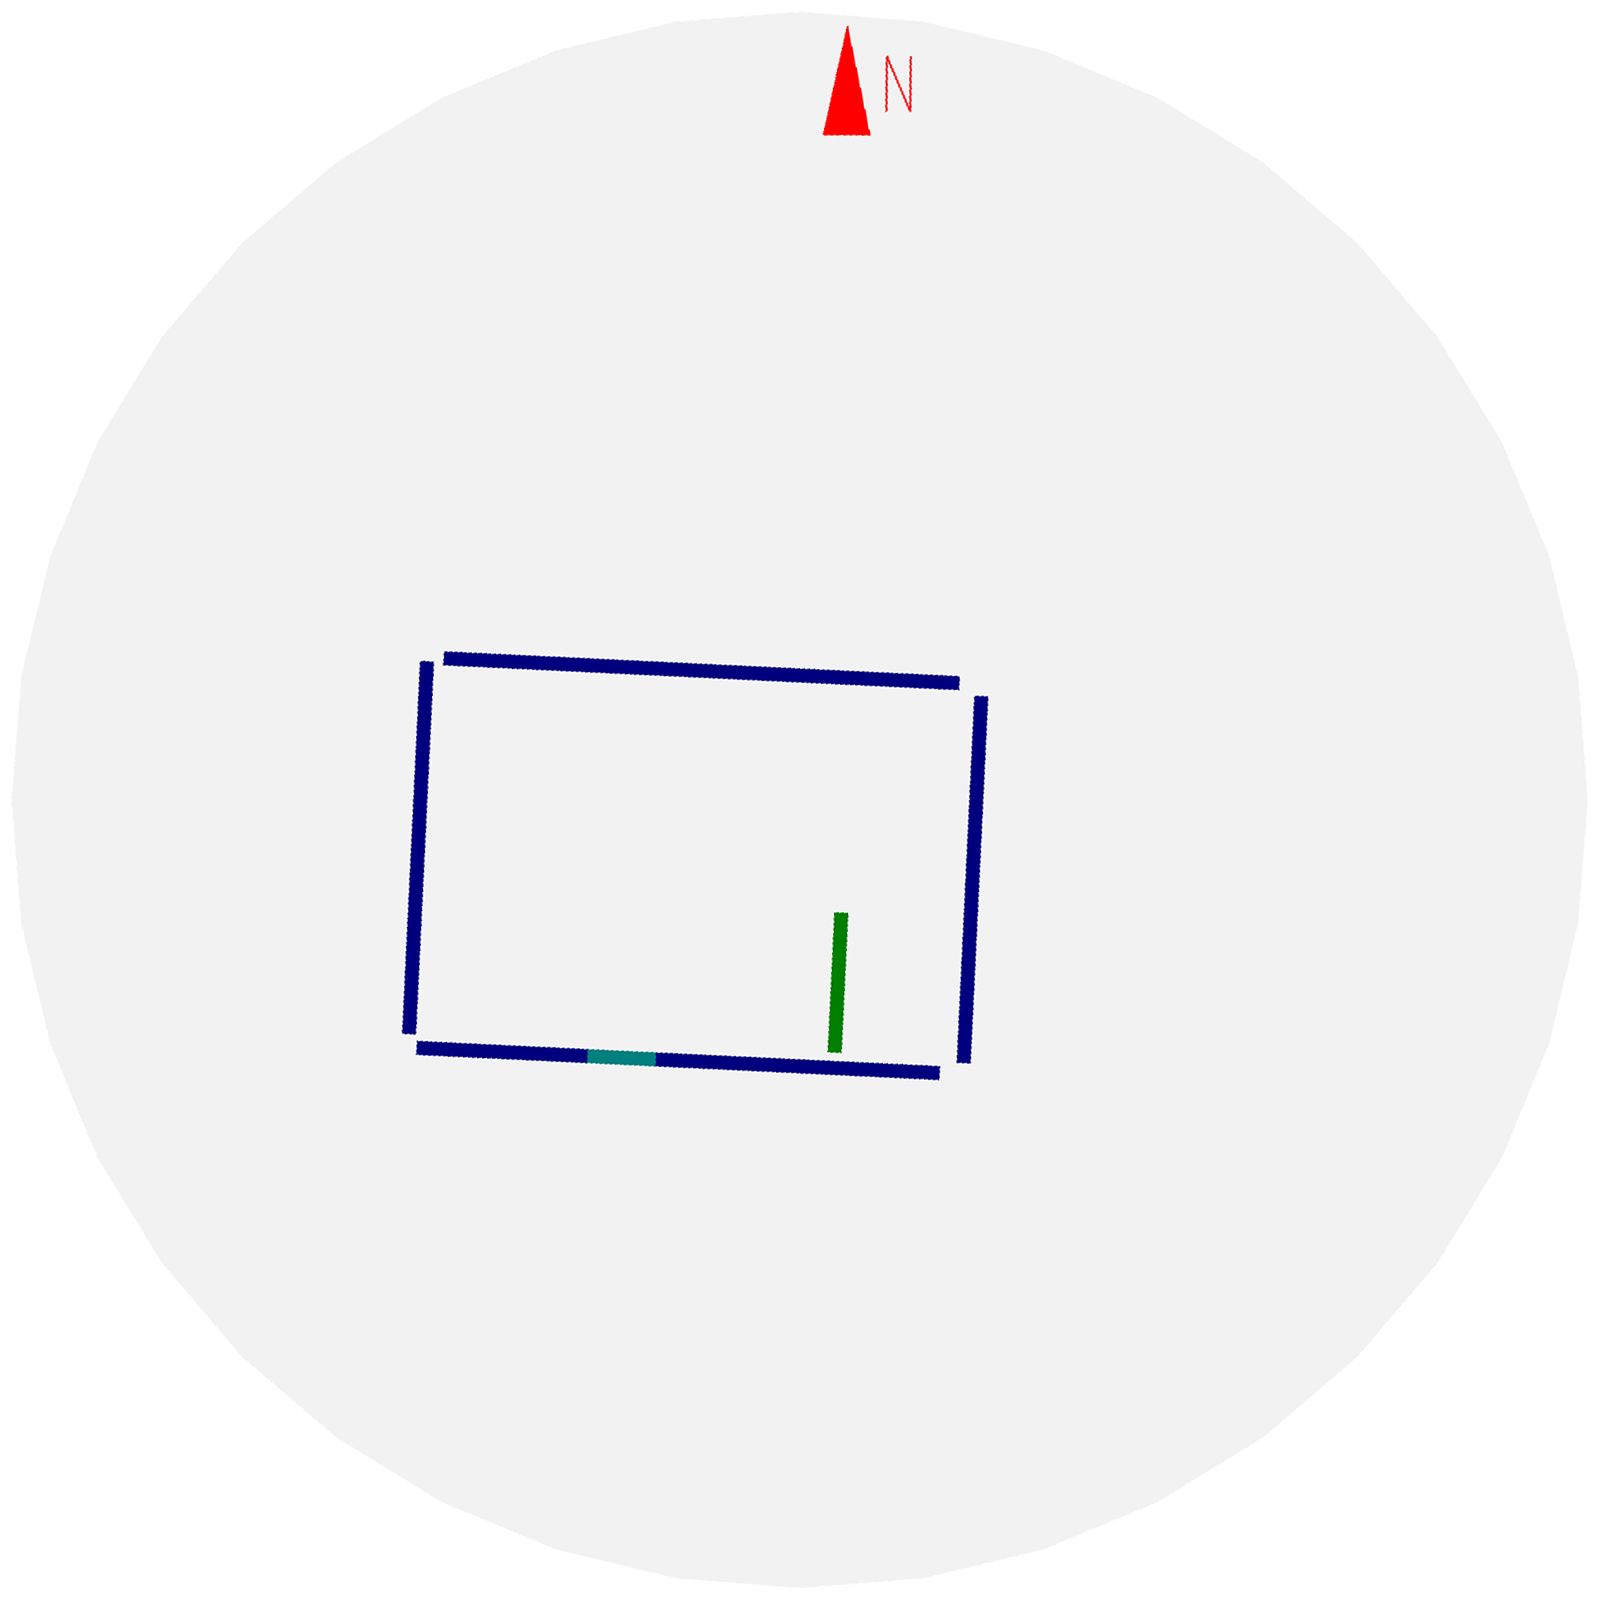
\includegraphics[width=0.19\columnwidth]{../gi2012_userstudy/images/section2/3_2D_walls_rotate} %N2
  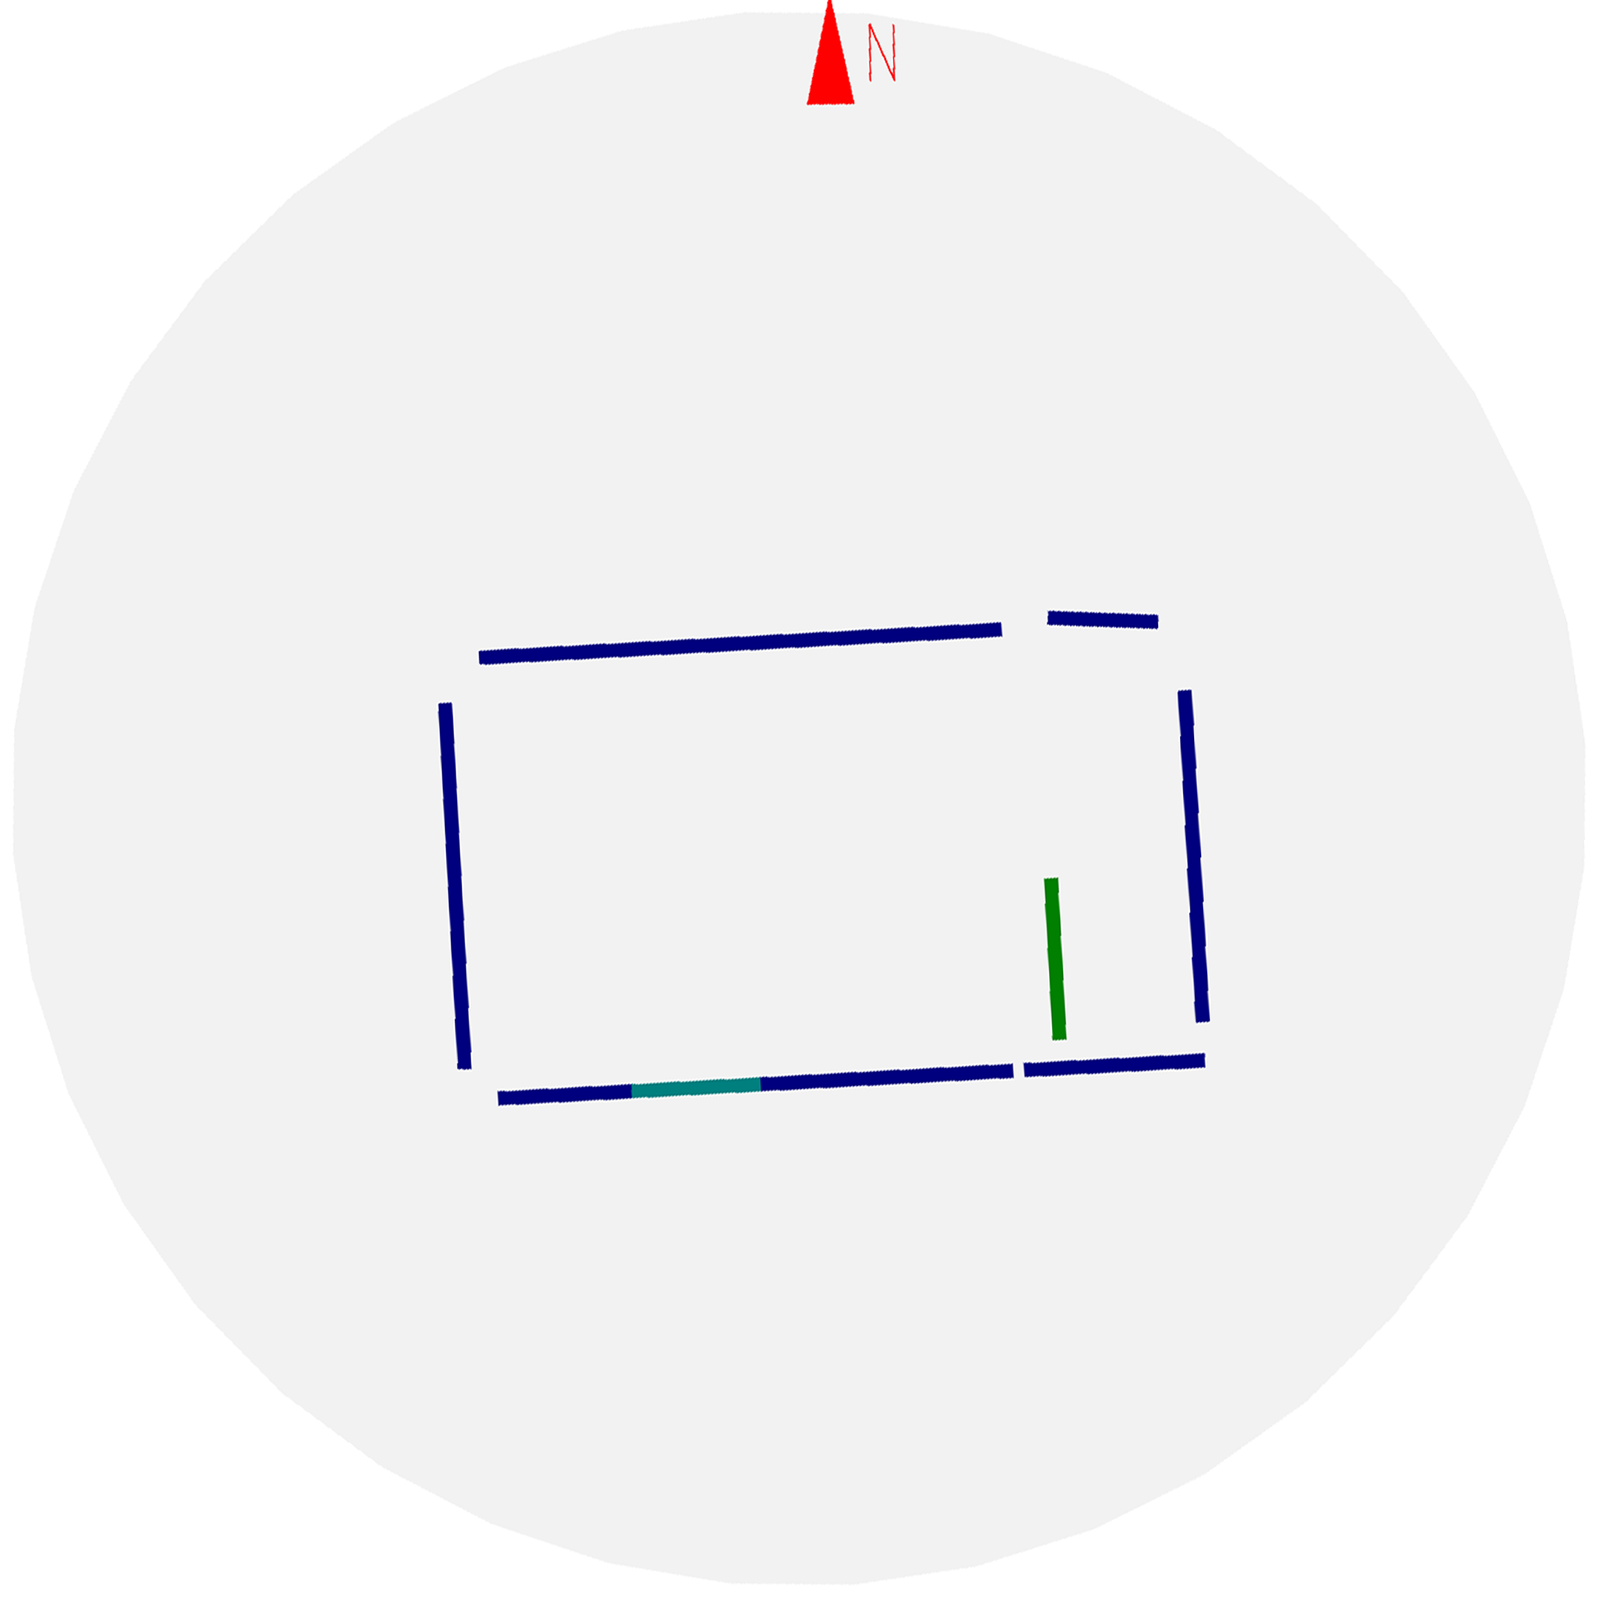
\includegraphics[width=0.19\columnwidth]{../gi2012_userstudy/images/section2/5_2D_walls_rotate} %N4
  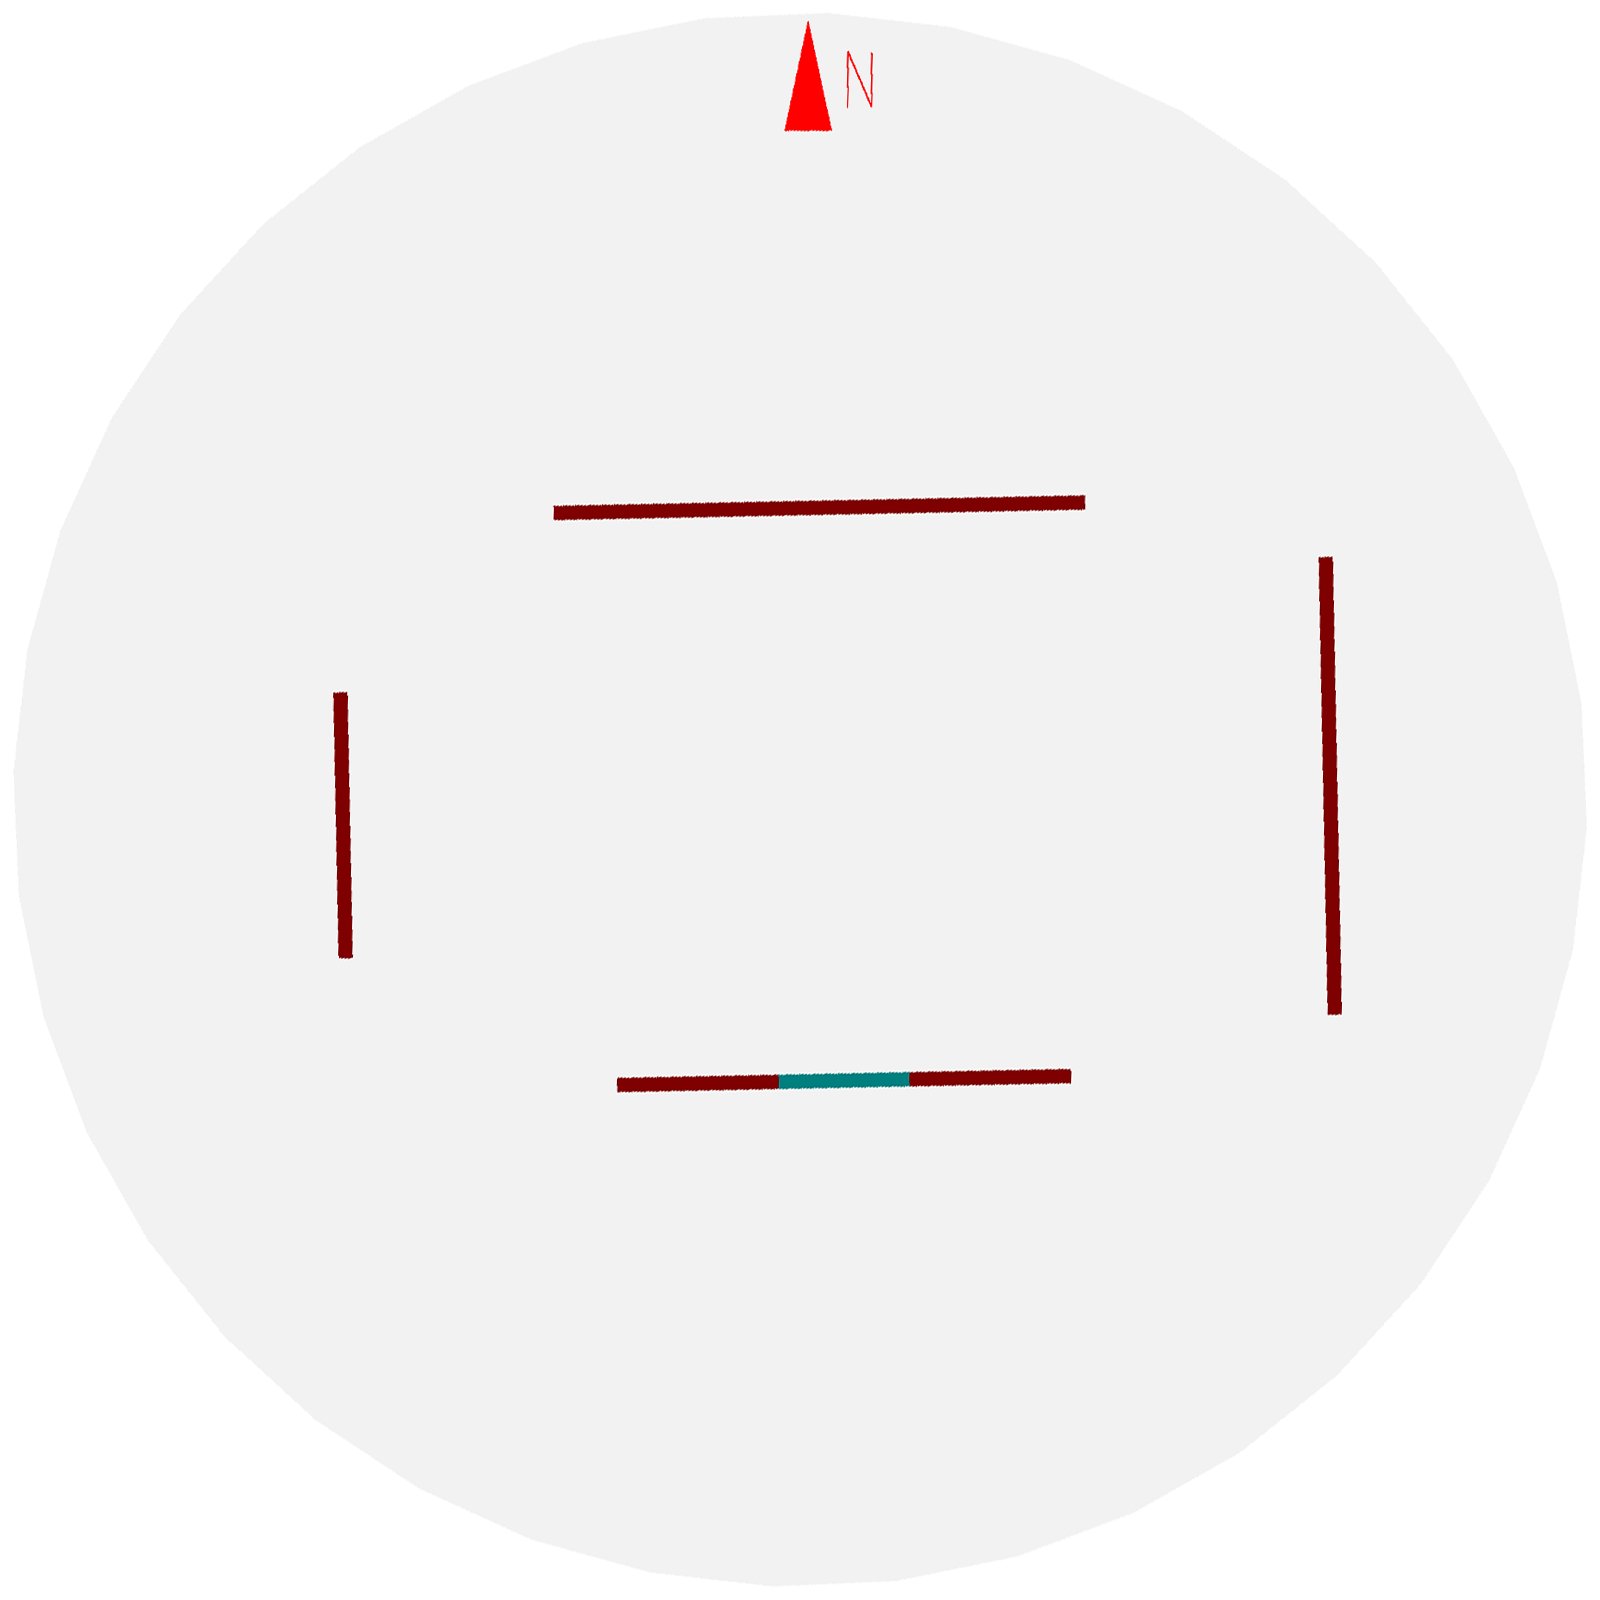
\includegraphics[width=0.19\columnwidth]{../gi2012_userstudy/images/section2/9_2D_walls_rotate} %N5
  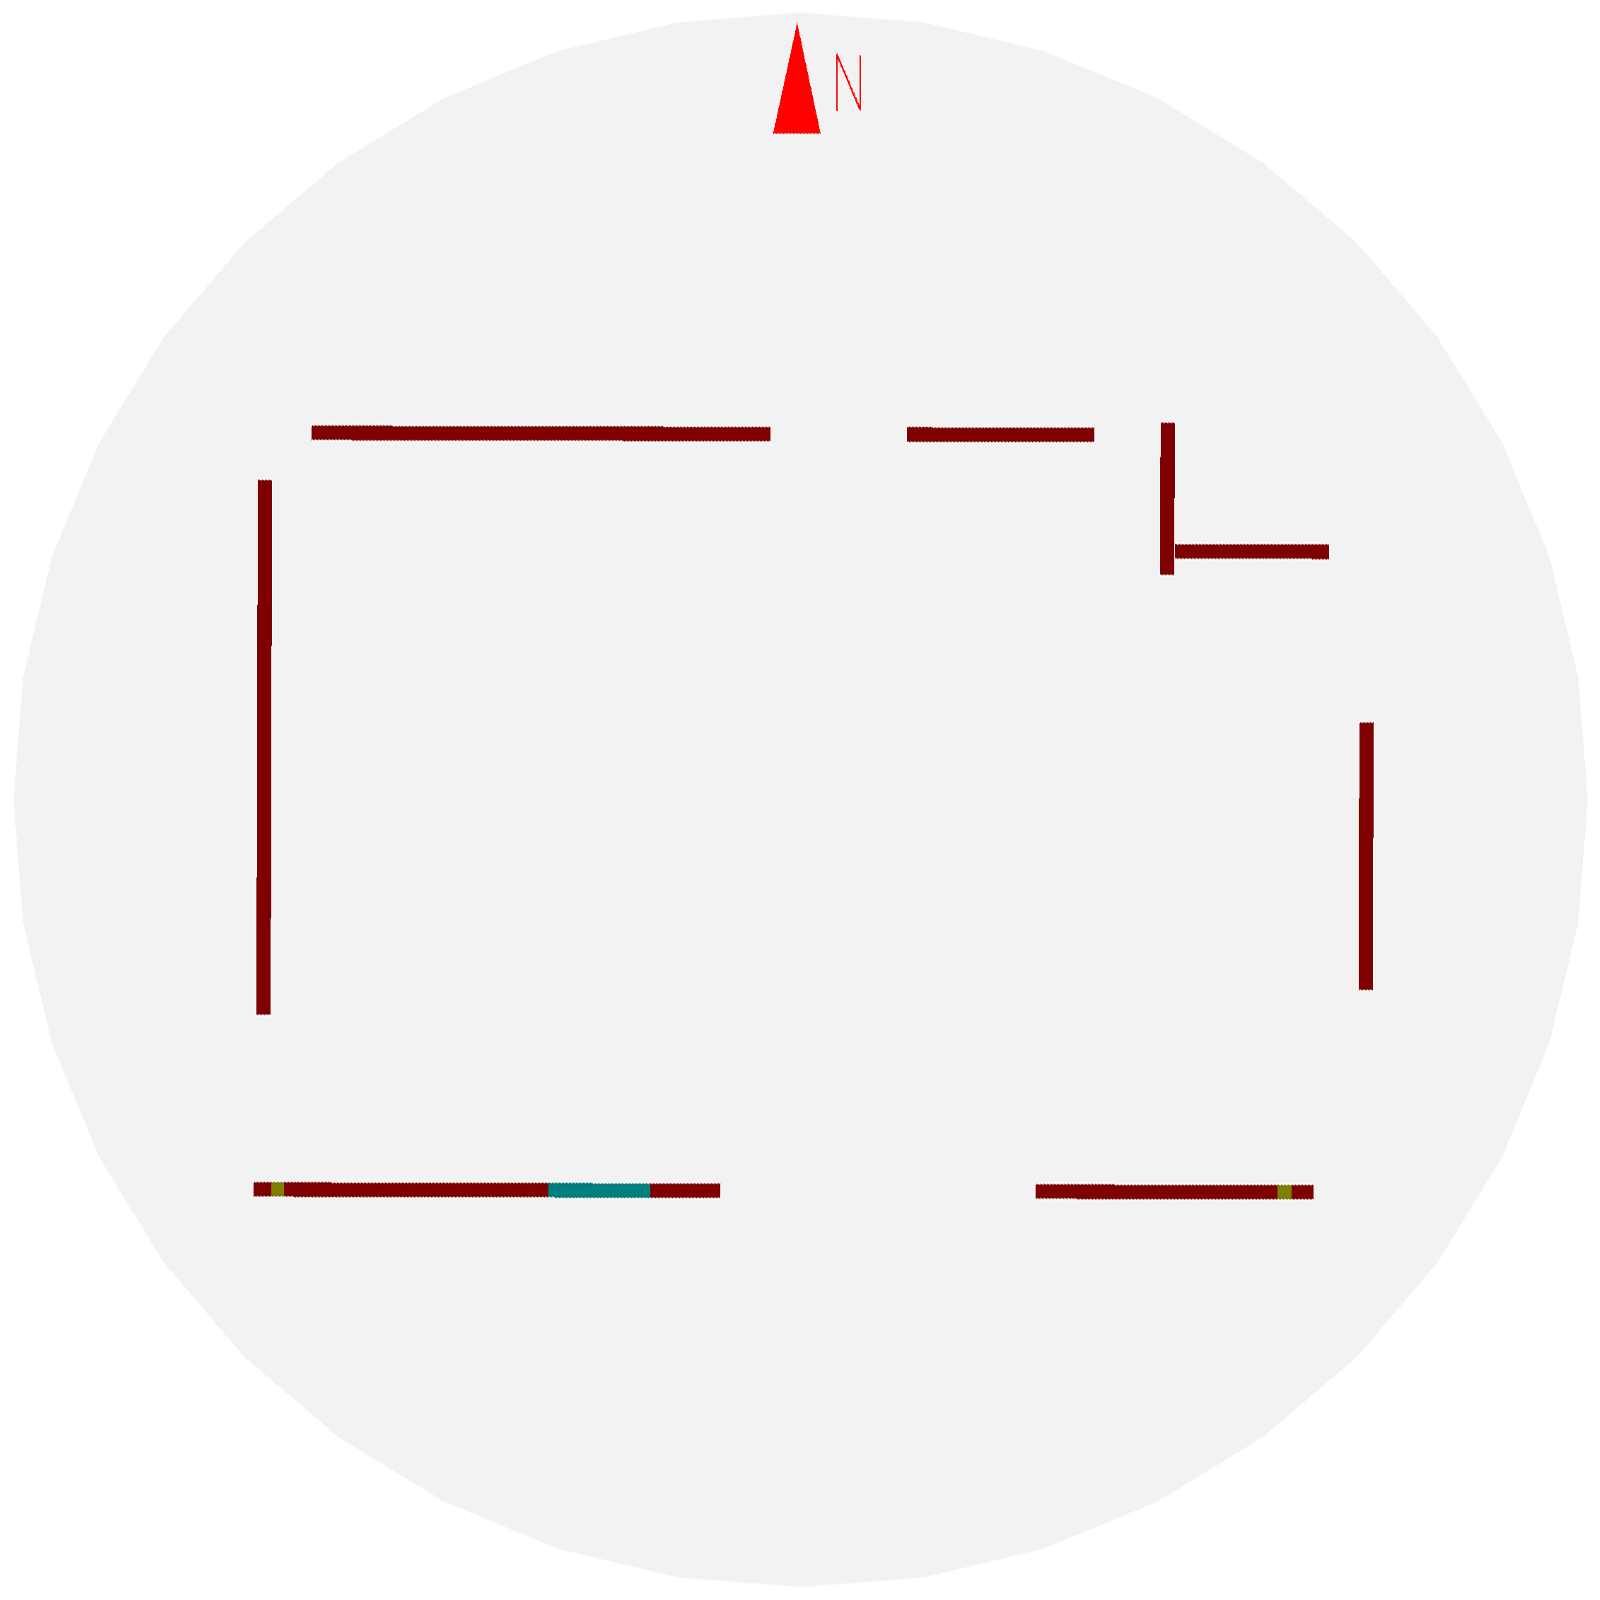
\includegraphics[width=0.19\columnwidth]{../gi2012_userstudy/images/section2/10_2D_walls_rotate} %N6\
  %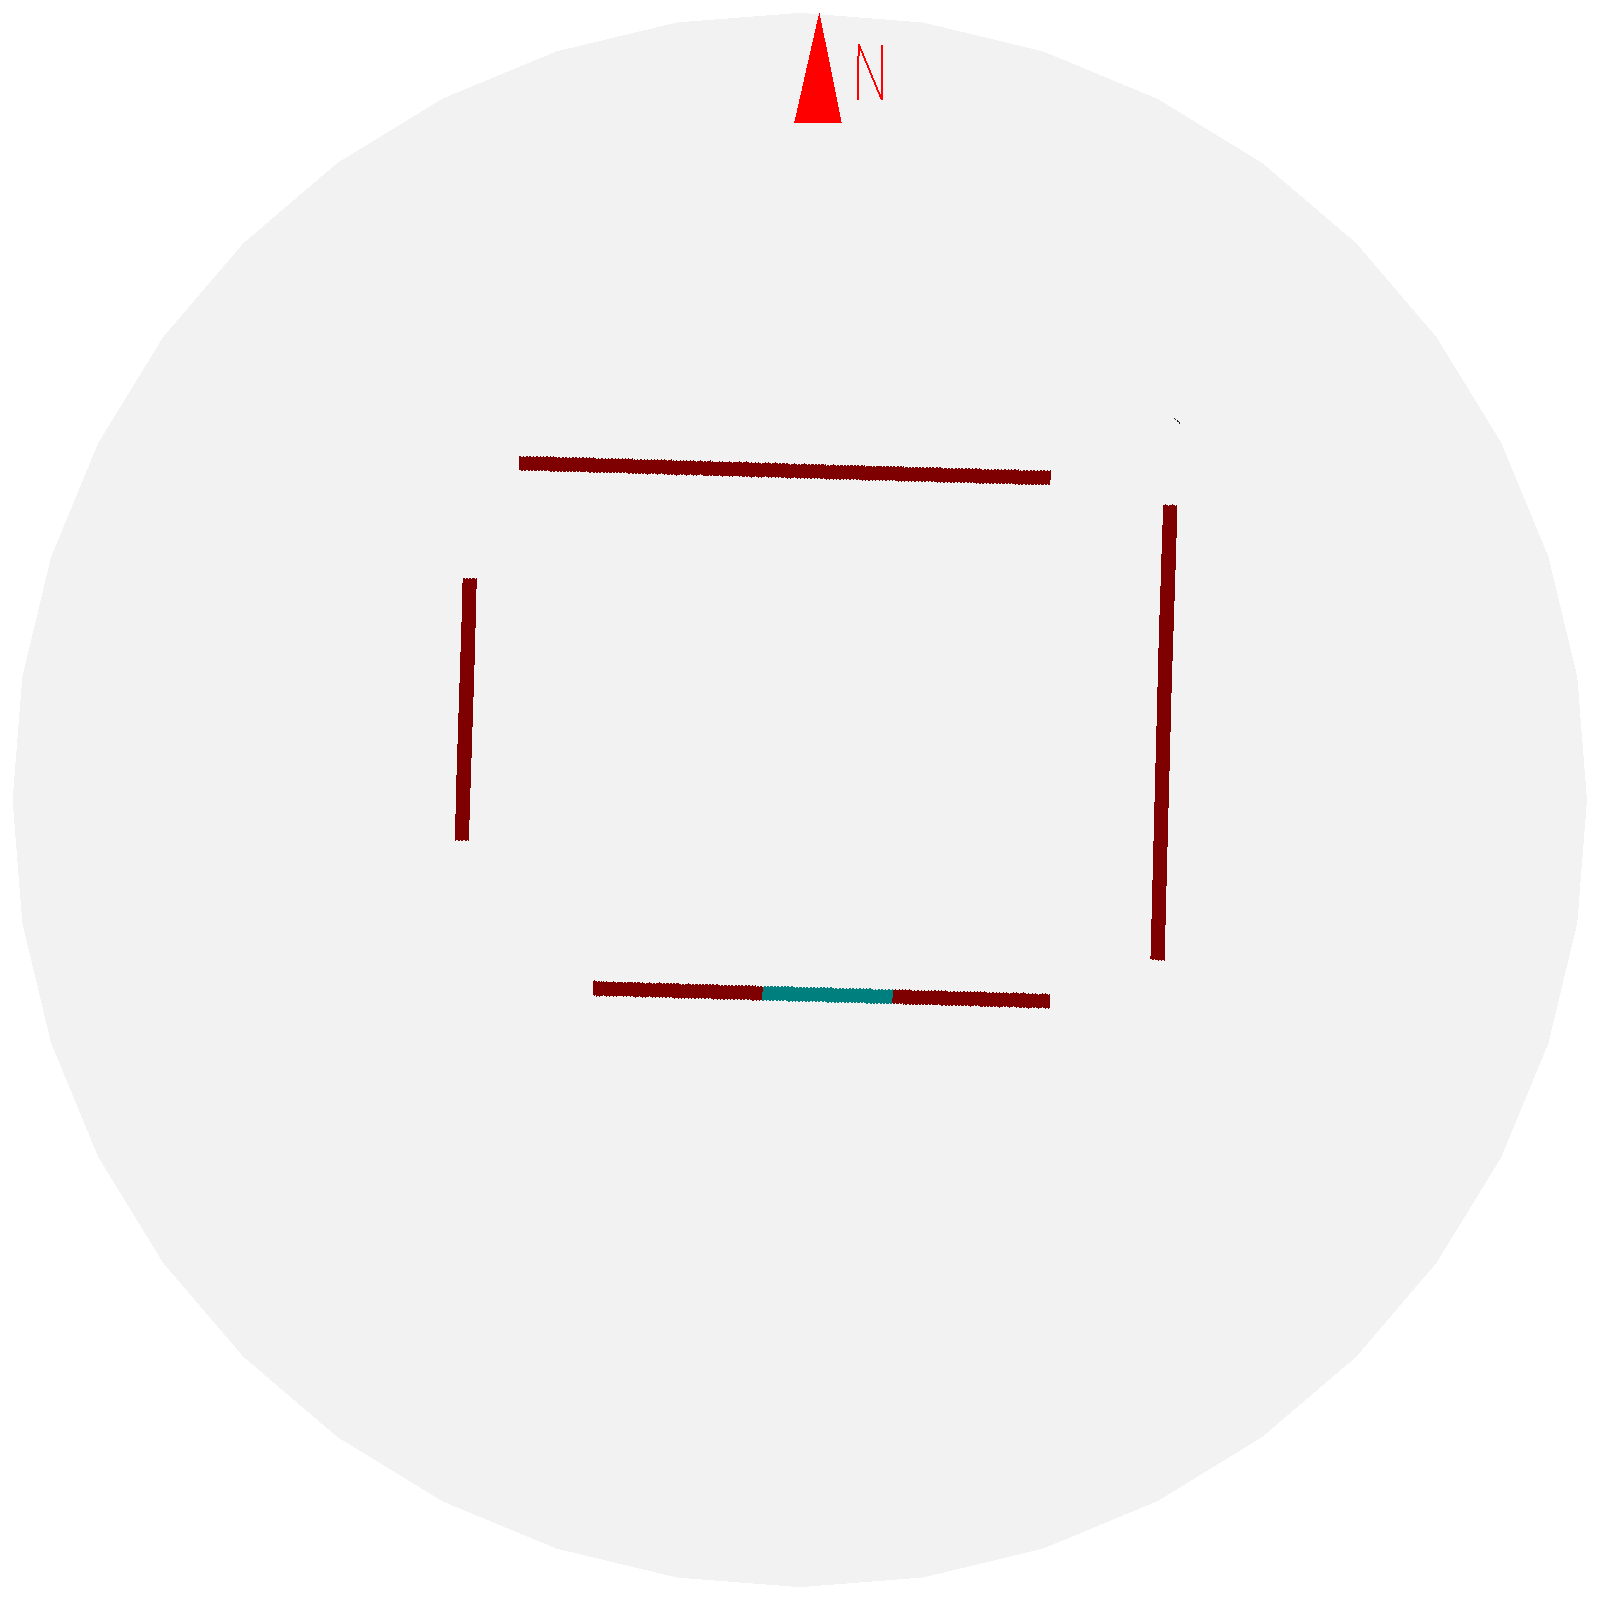
\includegraphics[width=0.2\columnwidth]{../gi2012_userstudy/images/section2/11_2D_walls_rotate} %N7
%} 
{\em \\
A photograph of the physical geometry of the original office space
constructed by one of the participants for Part 2 of the study and 2D
diagrams of the geometry constructed by the other participants.  Note
the variety of model complexity and scale that users create to
represent the same space.  The red walls are 10 inches tall and the
blue walls are 8 inches tall.
}

  %\hspace{.5in}
  \vspace{-6.8in}
\begin{minipage}{0.195\columnwidth}~{\color{white}{\bf N1}}\end{minipage} 
\begin{minipage}{0.195\columnwidth}~{\color{black}{\bf A1}}\end{minipage}
\begin{minipage}{0.195\columnwidth}~{\color{black}{\bf A2}}\end{minipage}
\begin{minipage}{0.195\columnwidth}~{\color{black}{\bf A4}}\end{minipage}
\begin{minipage}{0.195\columnwidth}~{\color{black}{\bf A5}}\end{minipage} \\
  \vspace{2.1in}
  
\begin{minipage}{0.195\columnwidth}~{\color{black}{\bf A6}}\end{minipage} 
\begin{minipage}{0.195\columnwidth}~{\color{black}{\bf N2}}\end{minipage}
\begin{minipage}{0.195\columnwidth}~{\color{black}{\bf N4}}\end{minipage}
\begin{minipage}{0.195\columnwidth}~{\color{black}{\bf N5}}\end{minipage}
\begin{minipage}{0.195\columnwidth}~{\color{black}{\bf N6}}\end{minipage} \\
\vspace{2.9in}
\\

\section*{Renovations to the Provided Space}
  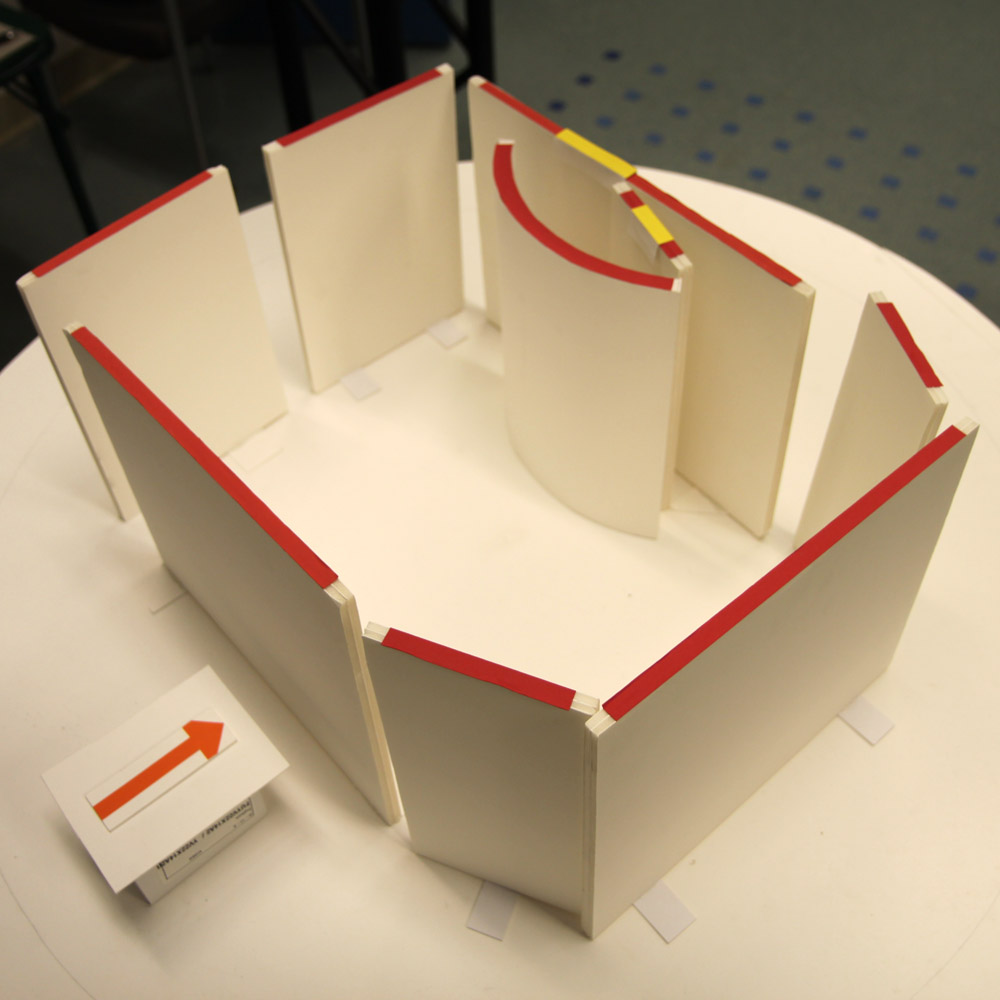
\includegraphics[width=0.19\columnwidth]{../gi2012_userstudy/images/photos/38_renovation} 
  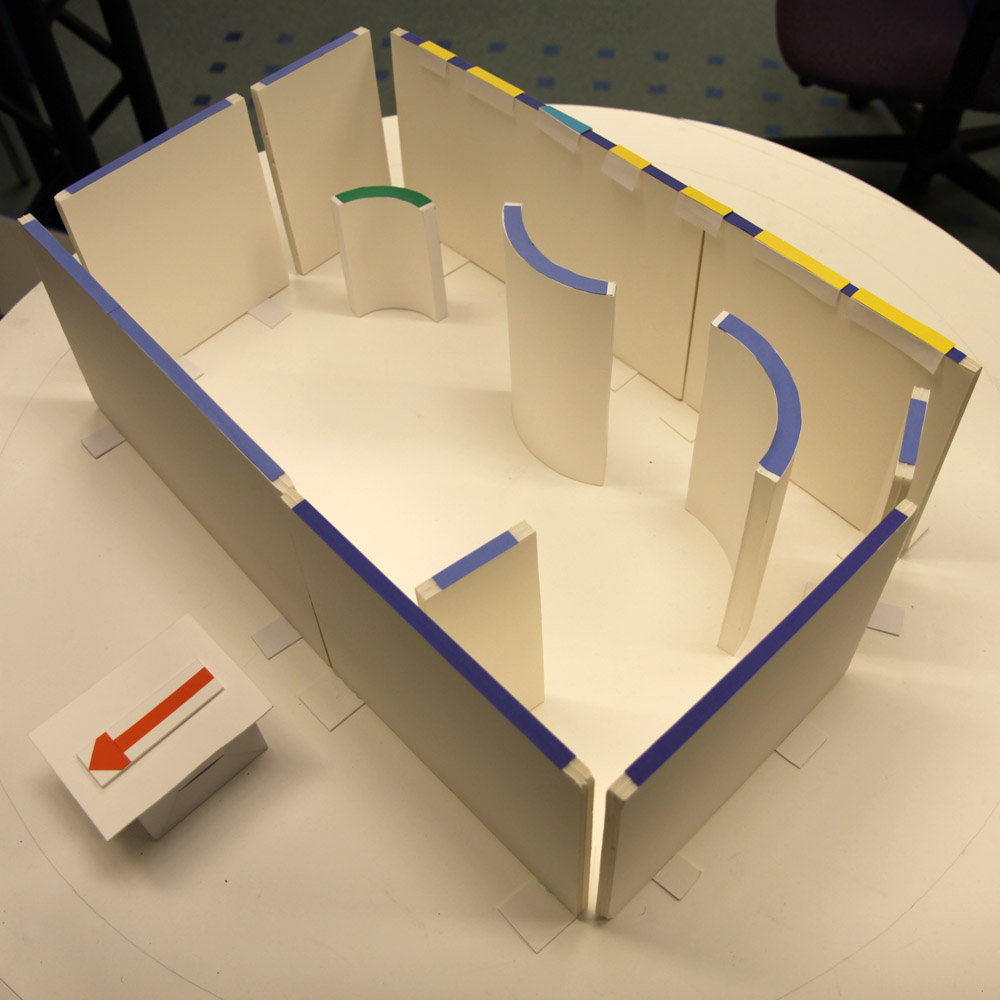
\includegraphics[width=0.19\columnwidth]{../gi2012_userstudy/images/photos/42_renovation}
%\resizebox{0.7\columnwidth}{!}{ 
  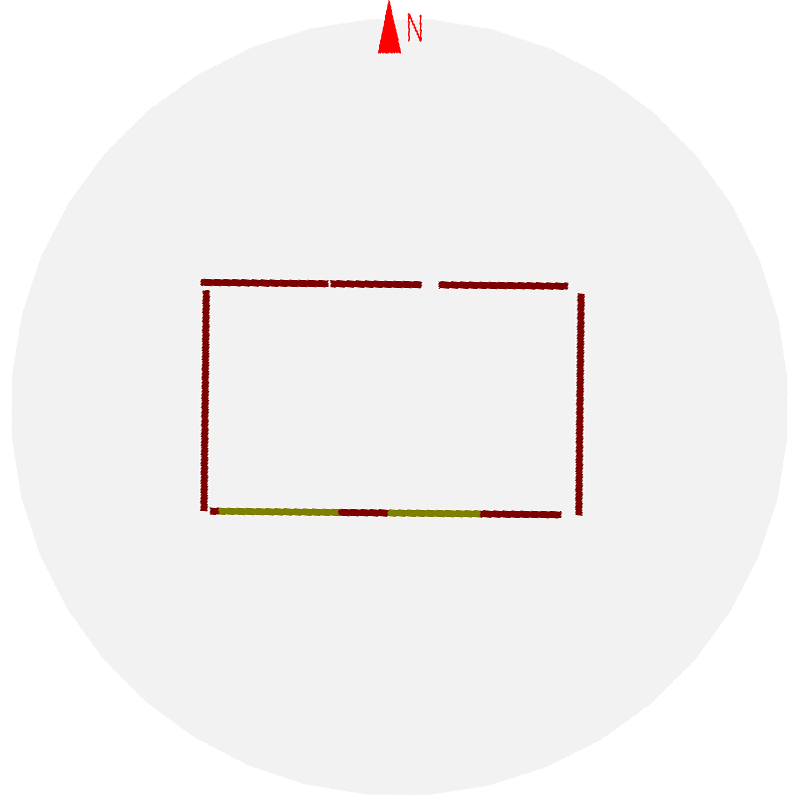
\includegraphics[width=0.19\columnwidth]{../gi2012_userstudy/images/section3/0_2D_walls_rotate_edit} %A1
  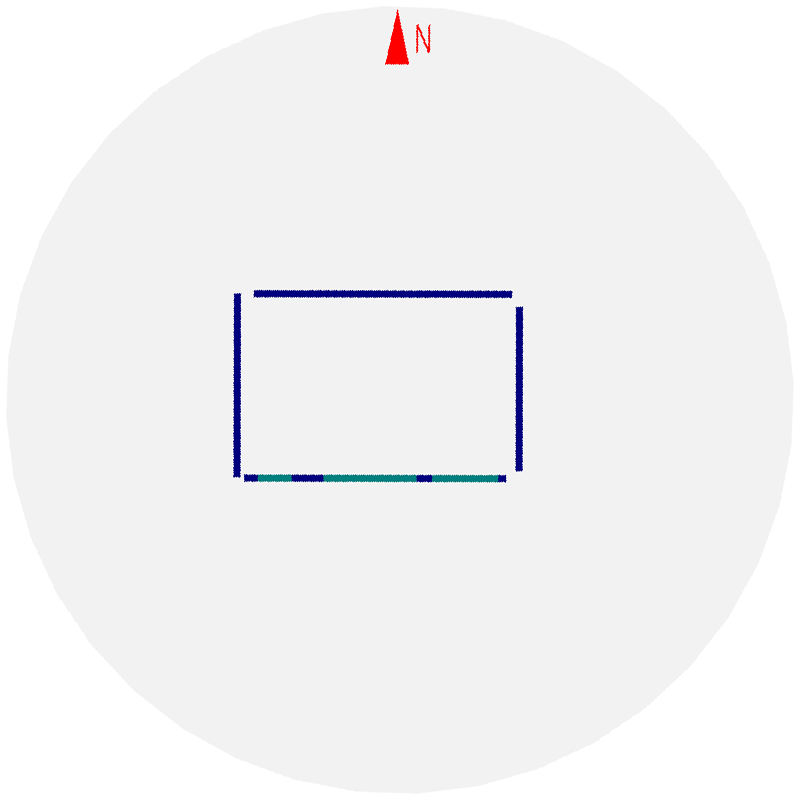
\includegraphics[width=0.19\columnwidth]{../gi2012_userstudy/images/section3/6_2D_walls_rotate} %A4
  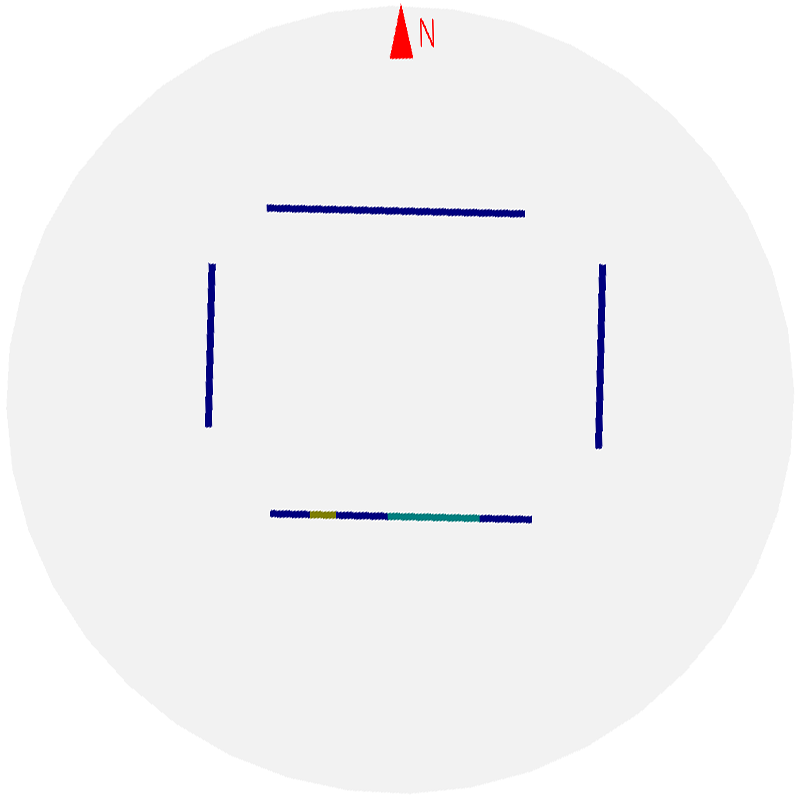
\includegraphics[width=0.19\columnwidth]{../gi2012_userstudy/images/section3/7_2D_walls_rotate}\\ %A5
  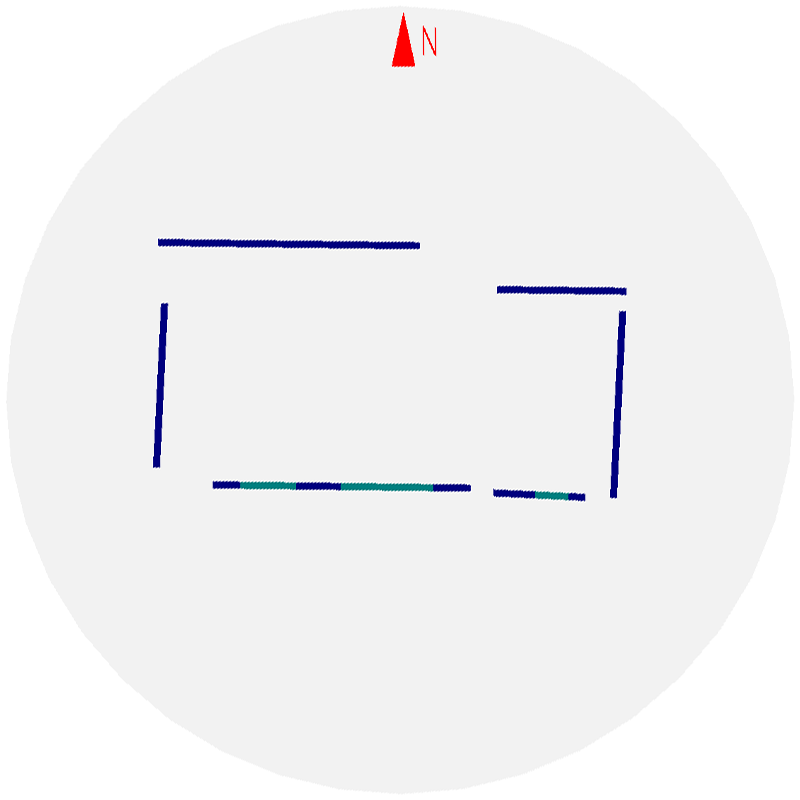
\includegraphics[width=0.19\columnwidth]{../gi2012_userstudy/images/section3/8_2D_walls_rotate} %A6
  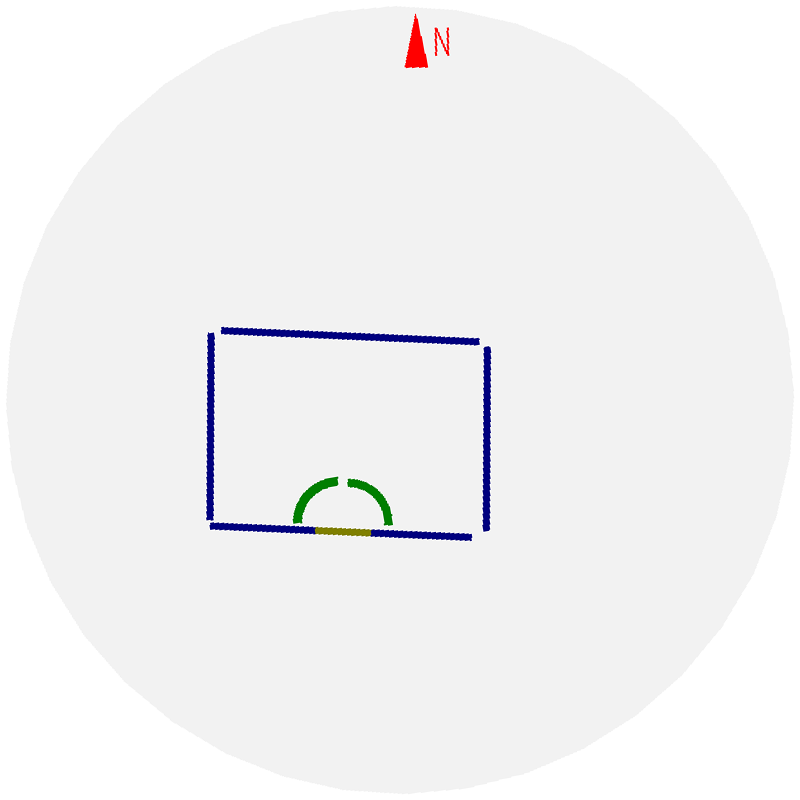
\includegraphics[width=0.19\columnwidth]{../gi2012_userstudy/images/section3/2_2D_walls_rotate} %N2
  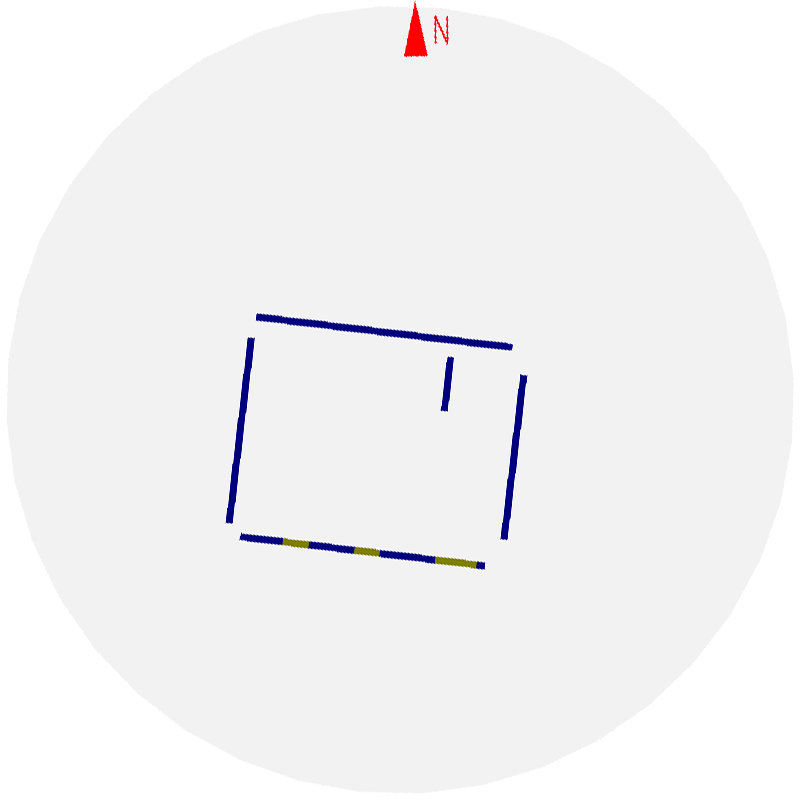
\includegraphics[width=0.19\columnwidth]{../gi2012_userstudy/images/section3/3_2D_walls_rotate} %N3
  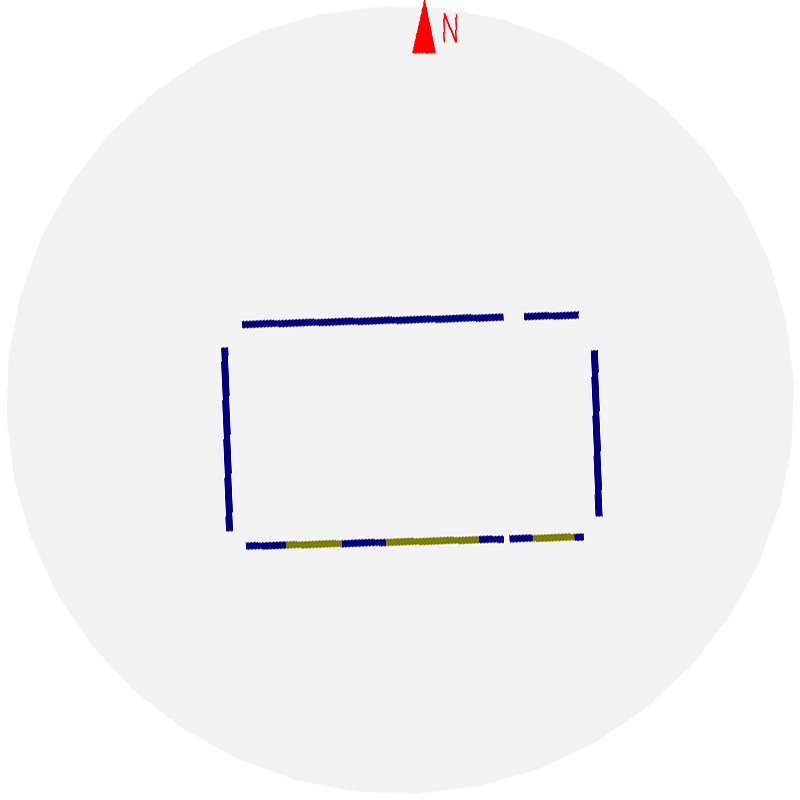
\includegraphics[width=0.19\columnwidth]{../gi2012_userstudy/images/section3/4_2D_walls_rotate} %N4
  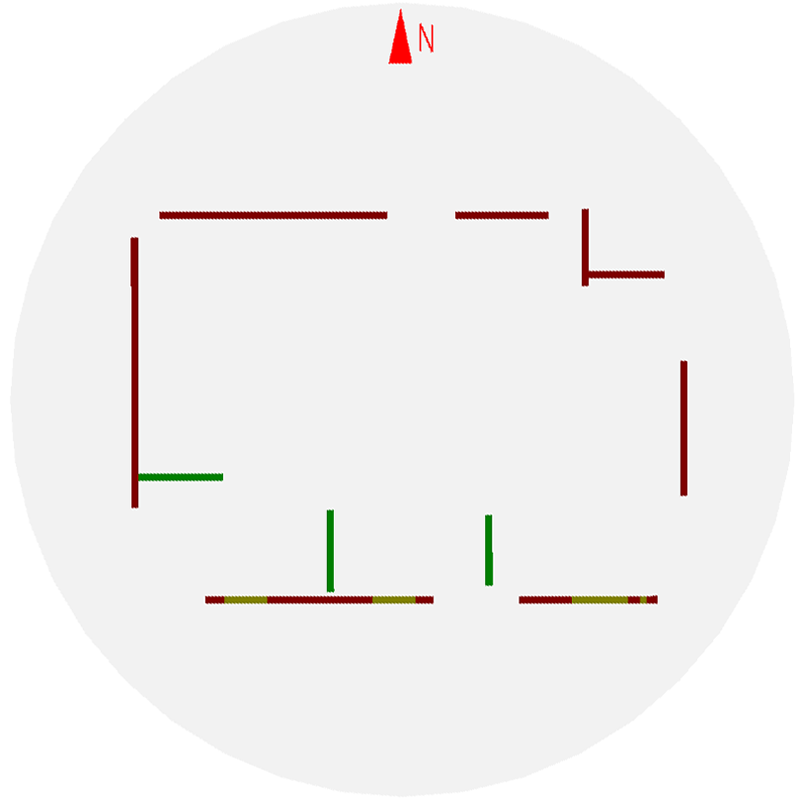
\includegraphics[width=0.19\columnwidth]{../gi2012_userstudy/images/section3/9_2D_walls_rotate} %N6
%} 
%
{\em
\\In Part 3 of the study participants were asked to propose
    a modest renovation to the geometry to improve the use of
    daylighting.  Some users simply added windows while others attempted
    to reduce glare.
}

  %\hspace{.5in}
  \vspace{-6.1in}
\begin{minipage}{0.195\columnwidth}~{\color{white}{\bf A2}}\end{minipage} 
\begin{minipage}{0.195\columnwidth}~{\color{white}{\bf A3}}\end{minipage}
\begin{minipage}{0.195\columnwidth}~{\color{black}{\bf A1}}\end{minipage}
\begin{minipage}{0.195\columnwidth}~{\color{black}{\bf A4}}\end{minipage}
\begin{minipage}{0.195\columnwidth}~{\color{black}{\bf A5}}\end{minipage} \\
  \vspace{2.1in}
  
\begin{minipage}{0.195\columnwidth}~{\color{black}{\bf A6}}\end{minipage} 
\begin{minipage}{0.195\columnwidth}~{\color{black}{\bf N2}}\end{minipage}
\begin{minipage}{0.195\columnwidth}~{\color{black}{\bf N4}}\end{minipage}
\begin{minipage}{0.195\columnwidth}~{\color{black}{\bf N5}}\end{minipage}
\begin{minipage}{0.195\columnwidth}~{\color{black}{\bf N6}}\end{minipage} \\
\vspace{2.6in}
\\

{\small
\bibliographystyle{abbrv}
\nocite{ShengYYC09} 
\nocite{Raskar:2001:SLA}
\nocite{aag201015}
\bibliography{refs}
}
\end{minipage}
%
\hfill
%%%%%%%%%%%%%%%%%%%%%%%%%%%%%%%%%%%%%%%%%%%%%%%%%%%%%%%%%%%%%%%%%%%%%%%%%%%%%%%%%%%%%%%
\begin{minipage}[t]{17in}
%\\
\section*{Renderings using the Architectural Daylighting Tool}
\begin{tabular}{lc}
%
\begin{sideways}~~Camera 1\end{sideways}&
  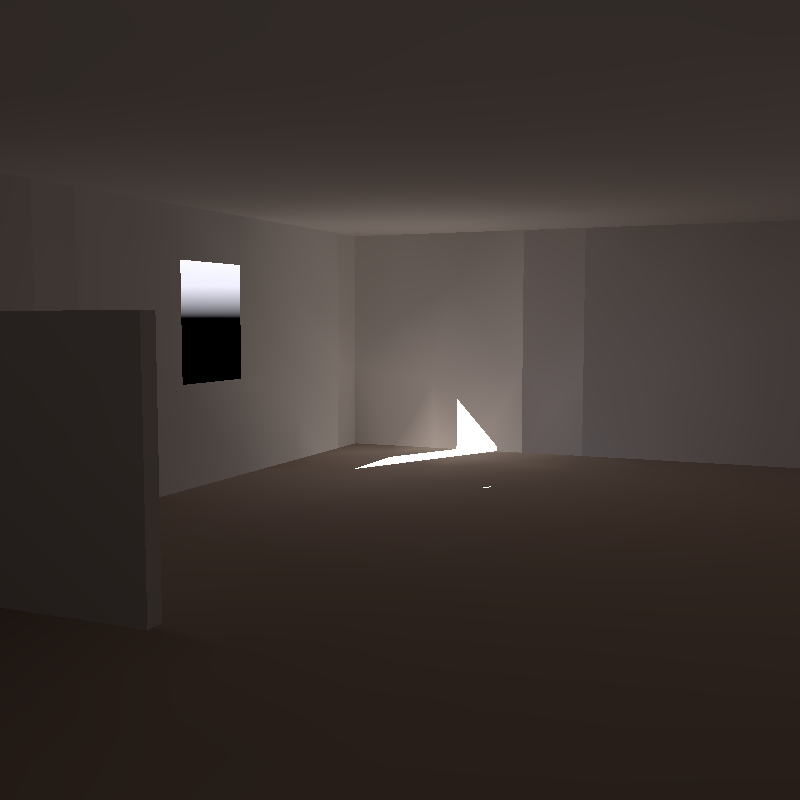
\includegraphics[width=0.158\textwidth]{../gi2012_userstudy/images/renderings/ground_truth/mrc331_camera_chris_march.png}
  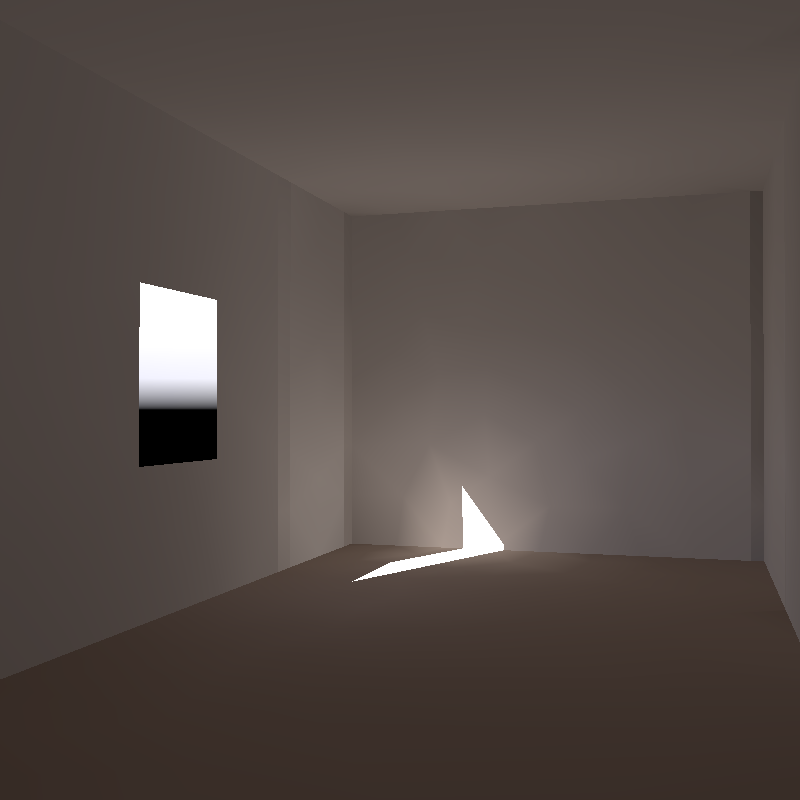
\includegraphics[width=0.158\textwidth]{../gi2012_userstudy/images/renderings/renovations/065_camera_chris_march.png}
  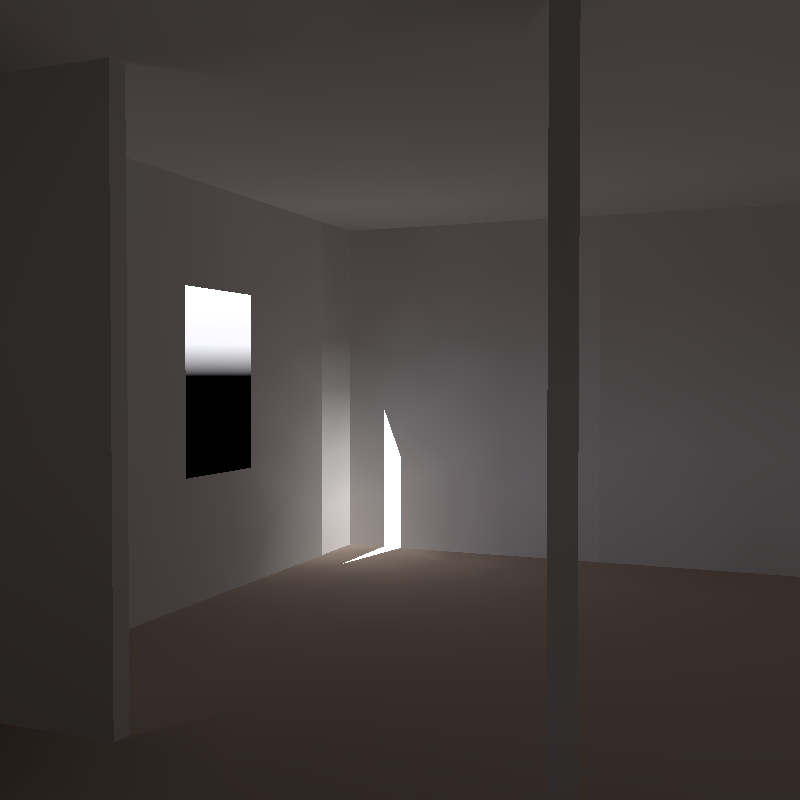
\includegraphics[width=0.158\textwidth]{../gi2012_userstudy/images/renderings/renovations/038_camera_chris_march.png}
  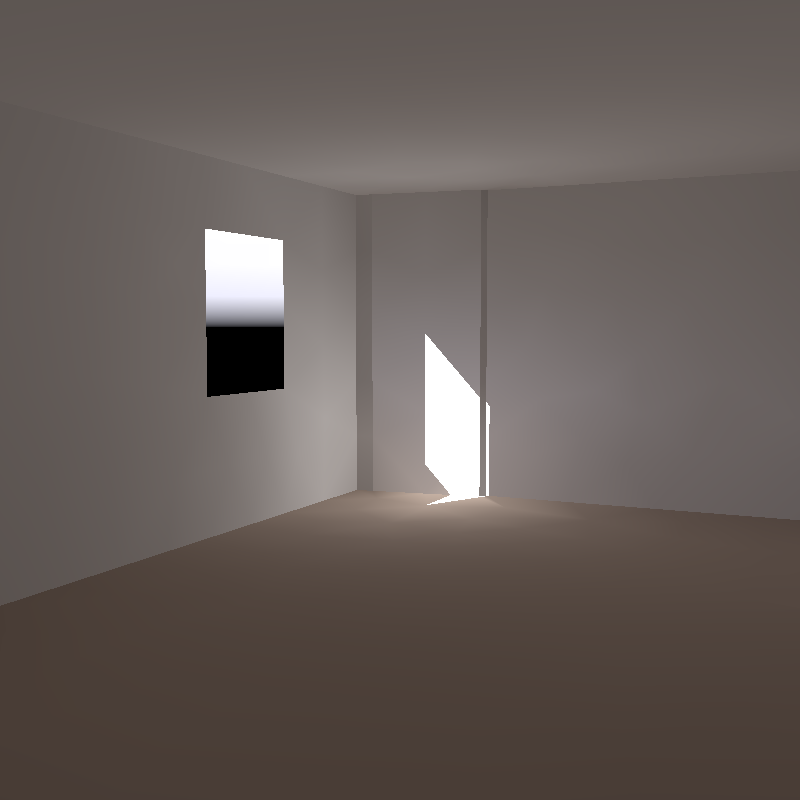
\includegraphics[width=0.158\textwidth]{../gi2012_userstudy/images/renderings/renovations/042_camera_chris_march.png}
  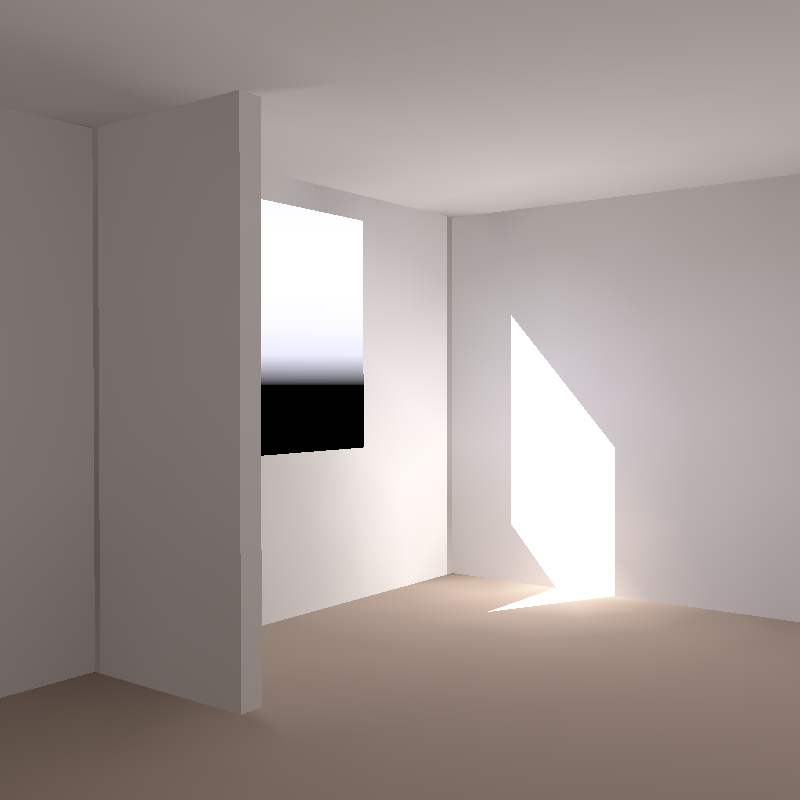
\includegraphics[width=0.158\textwidth]{../gi2012_userstudy/images/renderings/renovations/031_camera_chris_march.png}
  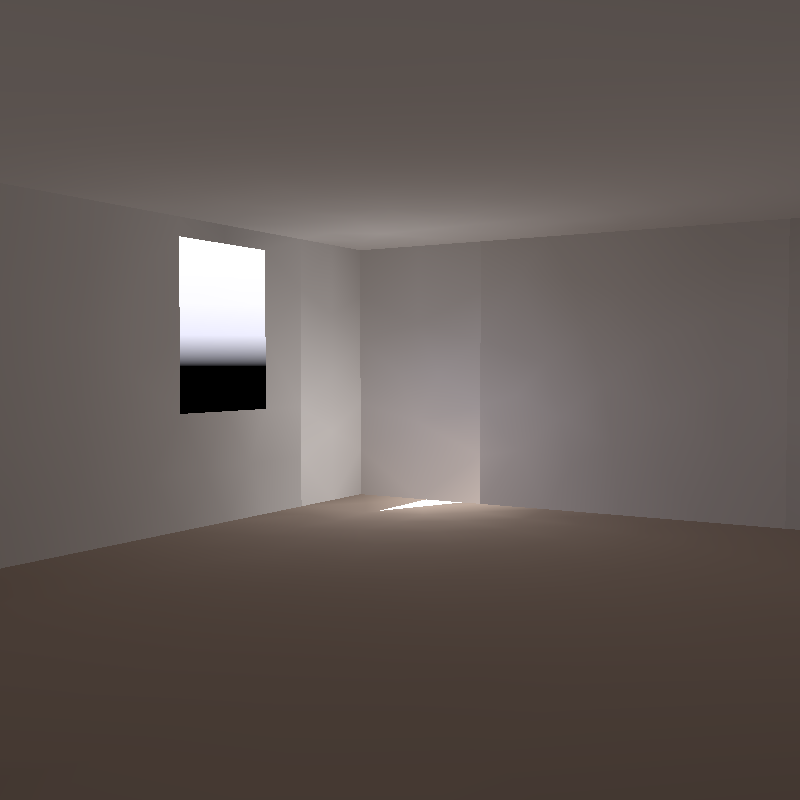
\includegraphics[width=0.158\textwidth]{../gi2012_userstudy/images/renderings/renovations/014_camera_chris_march.png}
\\
\begin{sideways}~~Camera 2\end{sideways}&
  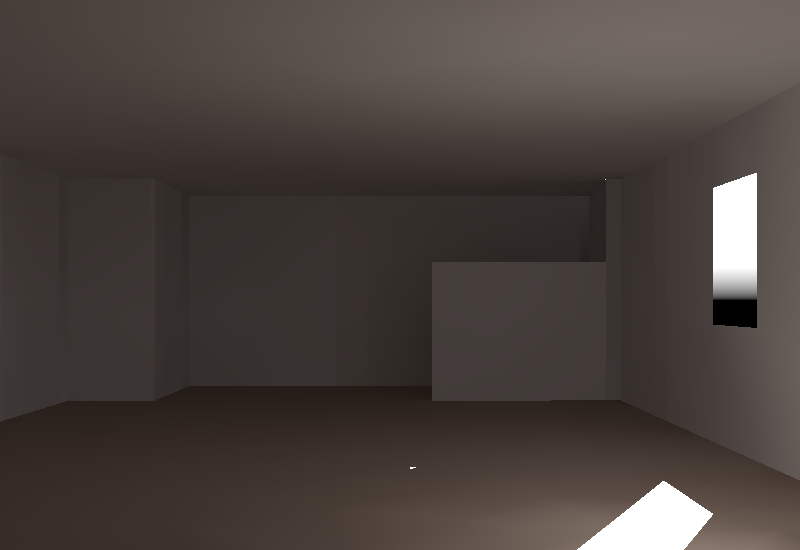
\includegraphics[width=0.158\textwidth]{../gi2012_userstudy/images/renderings/ground_truth/mrc331_camera_dark_march_crop.png}
  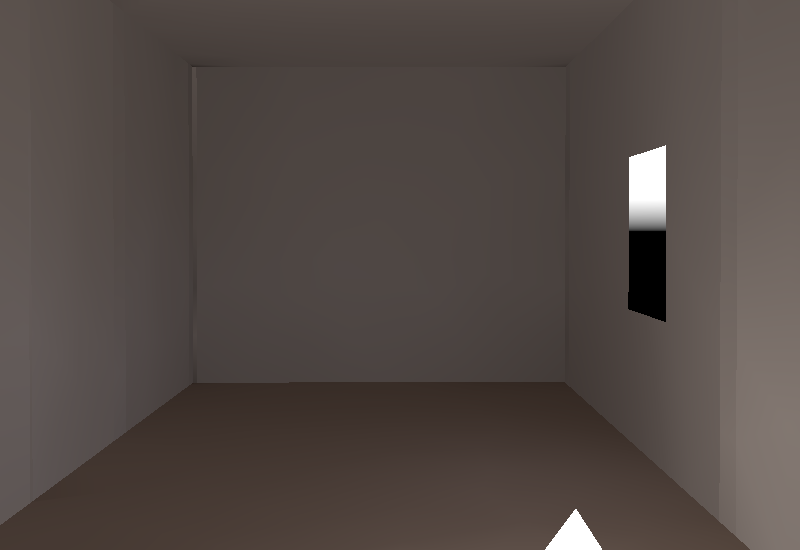
\includegraphics[width=0.158\textwidth]{../gi2012_userstudy/images/renderings/renovations/065_camera_dark_march_crop.png}
  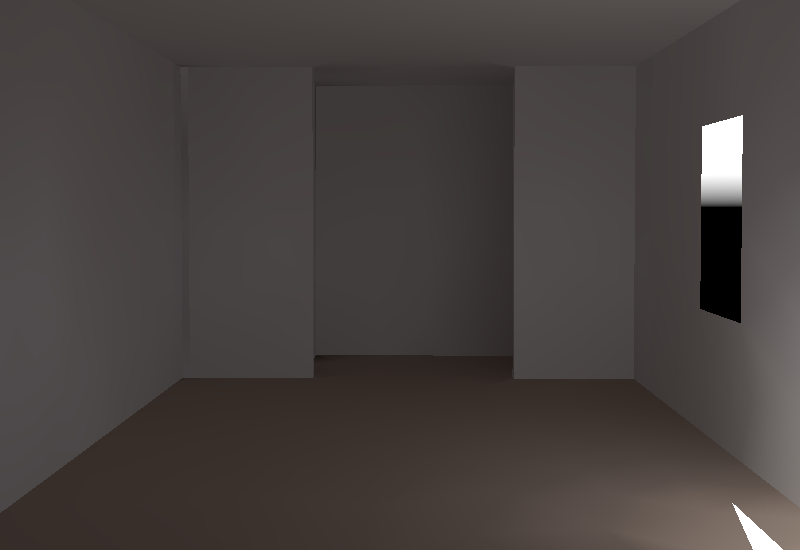
\includegraphics[width=0.158\textwidth]{../gi2012_userstudy/images/renderings/renovations/038_camera_dark_march_crop.png}
  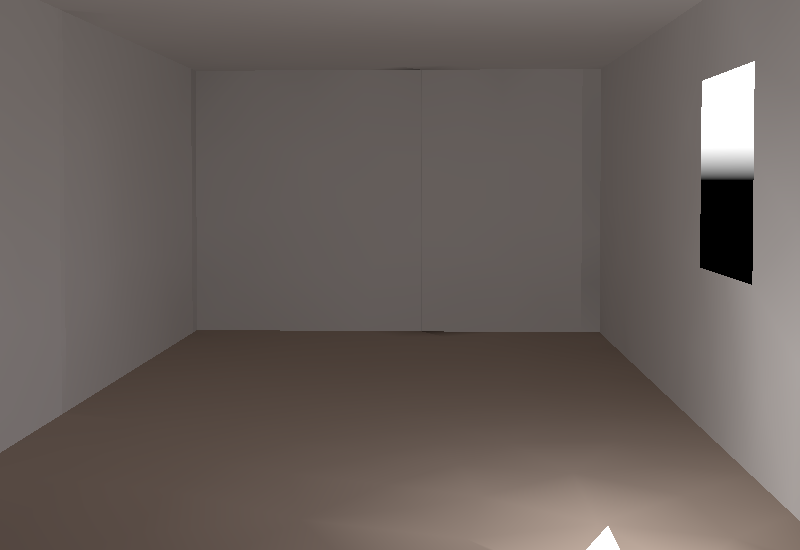
\includegraphics[width=0.158\textwidth]{../gi2012_userstudy/images/renderings/renovations/042_camera_dark_march_crop.png}
  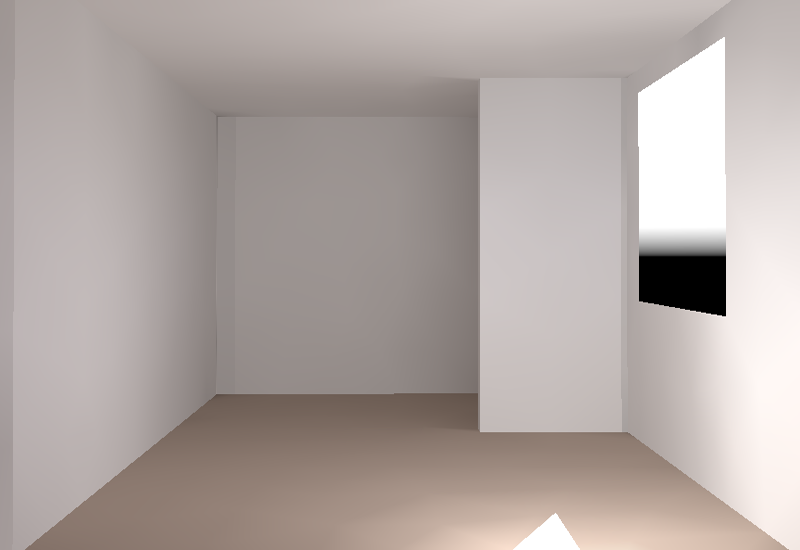
\includegraphics[width=0.158\textwidth]{../gi2012_userstudy/images/renderings/renovations/031_camera_dark_march_crop.png}
  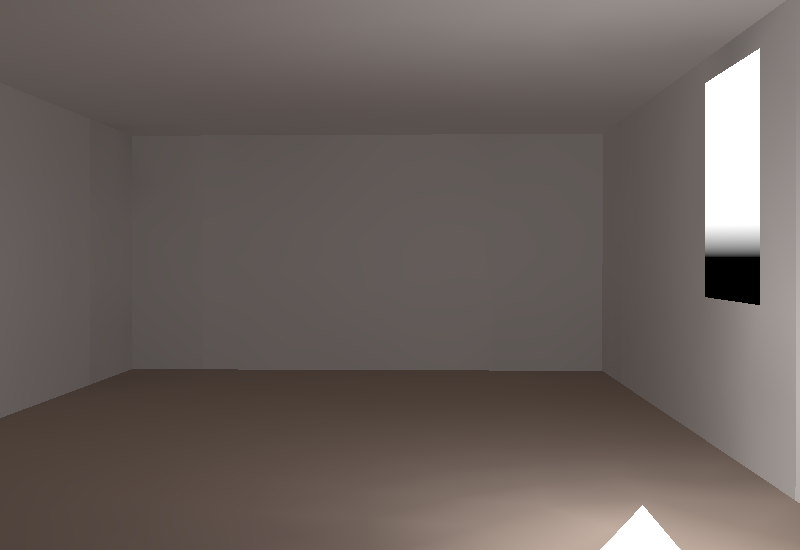
\includegraphics[width=0.158\textwidth]{../gi2012_userstudy/images/renderings/renovations/014_camera_dark_march_crop.png}\\
  \end{tabular}
  
  %\hspace{.5in}
  \vspace{-4.6in}
  %
  \hspace{.5in}
\begin{minipage}{0.158\textwidth}~{\color{white}{\bf ground-truth}}\end{minipage} 
\begin{minipage}{0.158\textwidth}~{\color{white}{\bf A1}}\end{minipage}
\begin{minipage}{0.158\textwidth}~{\color{white}{\bf A2}}\end{minipage}
\begin{minipage}{0.158\textwidth}~{\color{white}{\bf A3}}\end{minipage}
\begin{minipage}{0.158\textwidth}~{\color{white}{\bf A4}}\end{minipage} 
\begin{minipage}{0.158\textwidth}~{\color{white}{\bf A5}}\end{minipage} \\
\vspace{4.2in}
\\
\begin{tabular}{lc}
\begin{sideways}~~Camera 1\end{sideways}&
  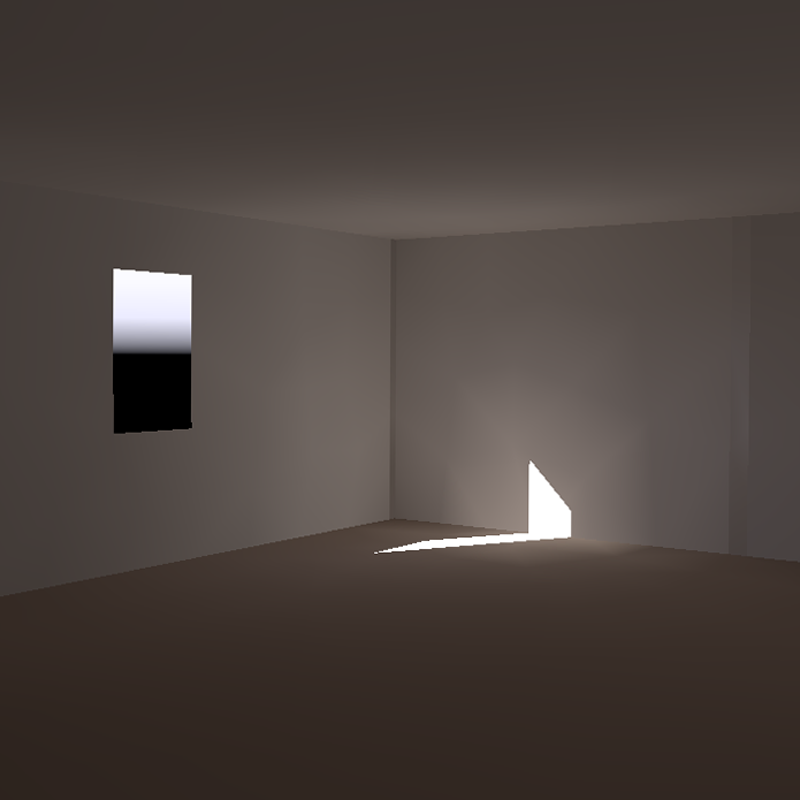
\includegraphics[width=0.158\textwidth]{../gi2012_userstudy/images/renderings/renovations/063_camera_chris_march_crop.png}
  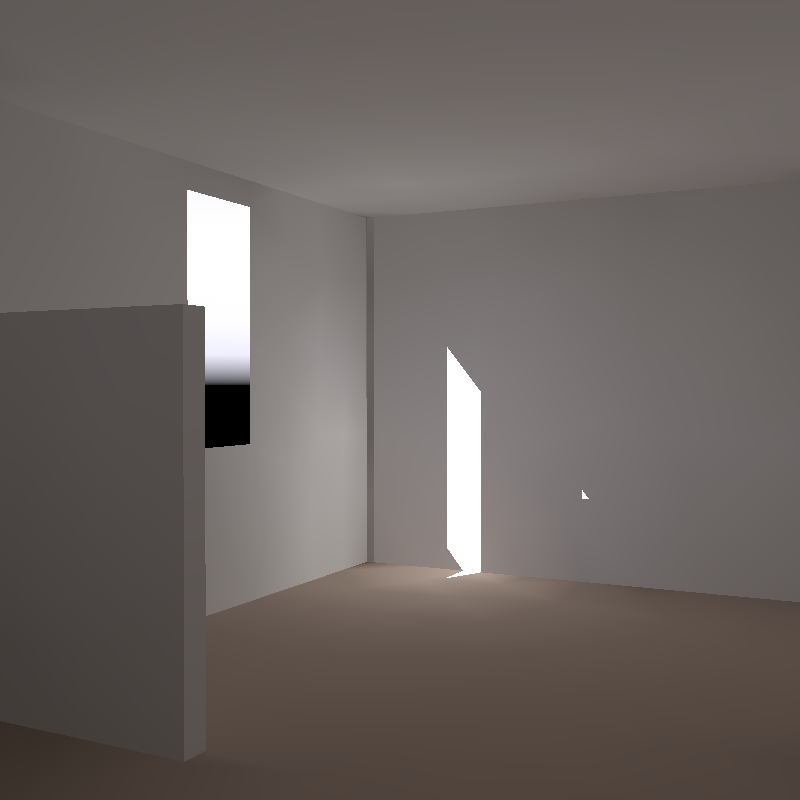
\includegraphics[width=0.158\textwidth]{../gi2012_userstudy/images/renderings/renovations/050_camera_chris_march.png}
  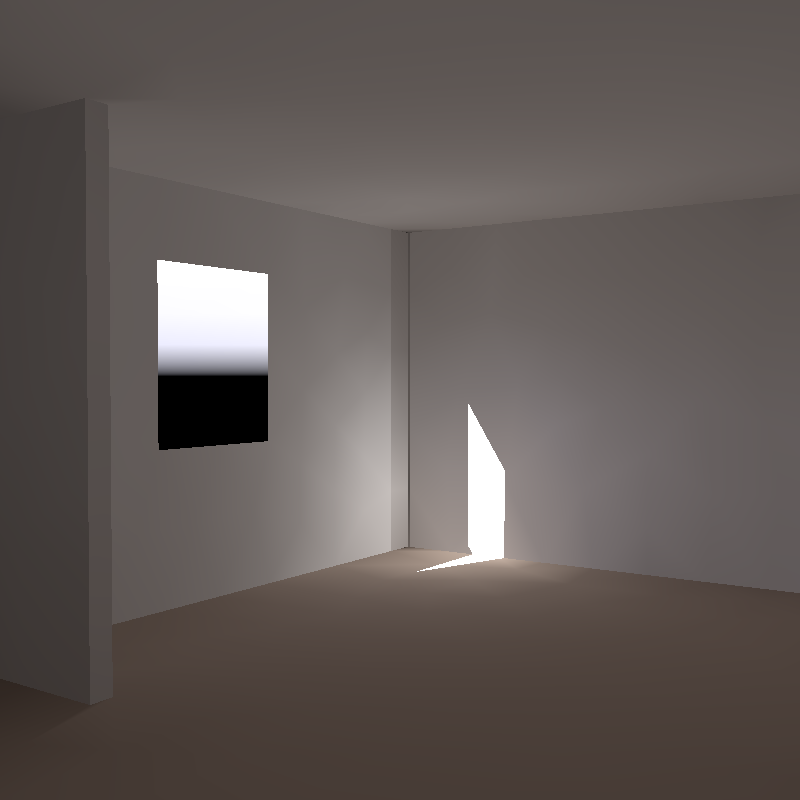
\includegraphics[width=0.158\textwidth]{../gi2012_userstudy/images/renderings/no_renovations/070_camera_chris_march.png}
  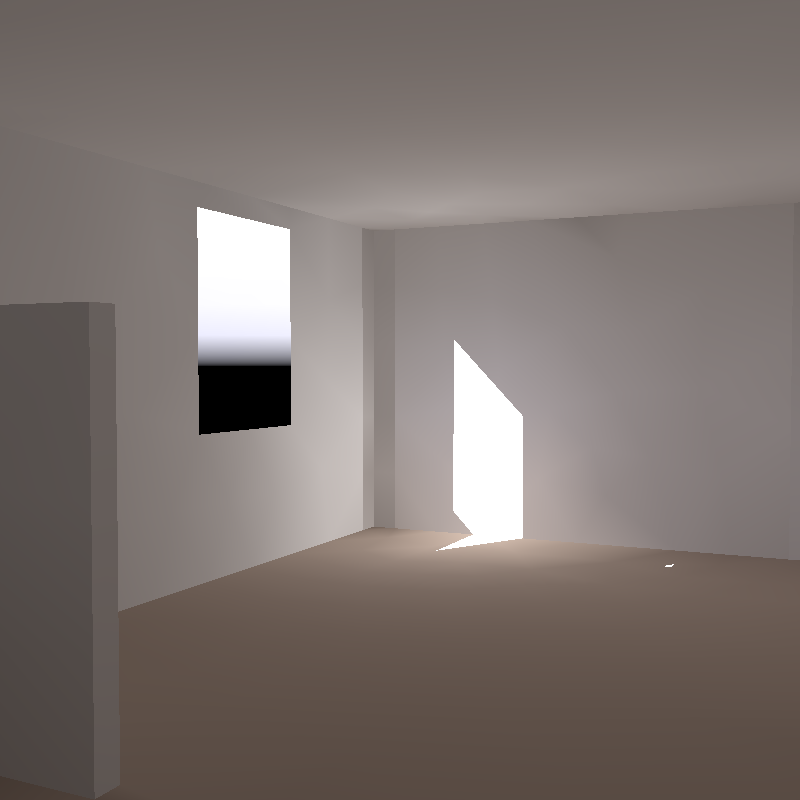
\includegraphics[width=0.158\textwidth]{../gi2012_userstudy/images/renderings/renovations/098_camera_chris_march.png}
  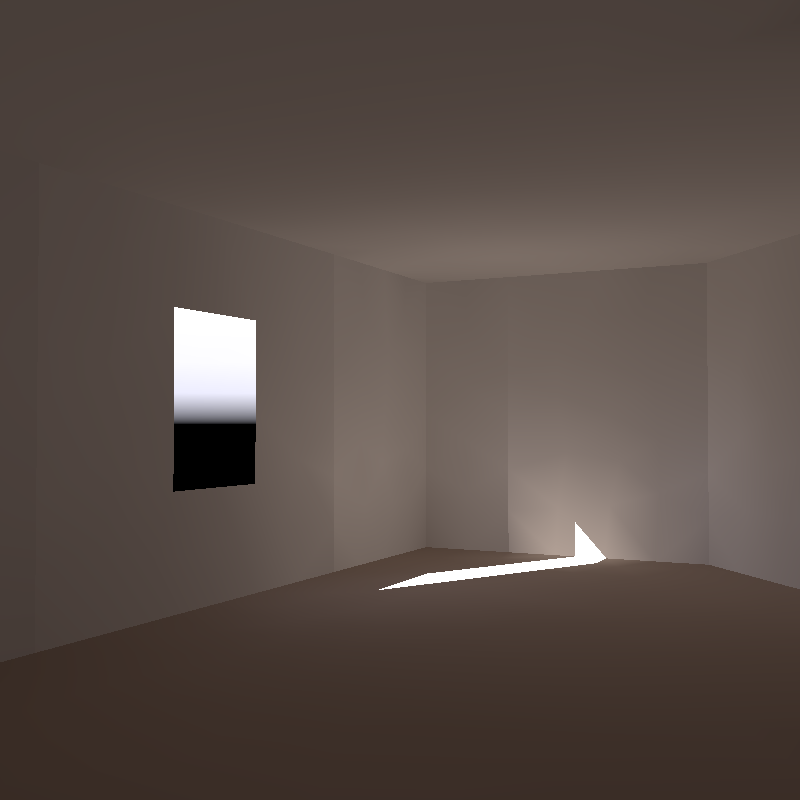
\includegraphics[width=0.158\textwidth]{../gi2012_userstudy/images/renderings/no_renovations/user_085_camera_chris_march.png}
  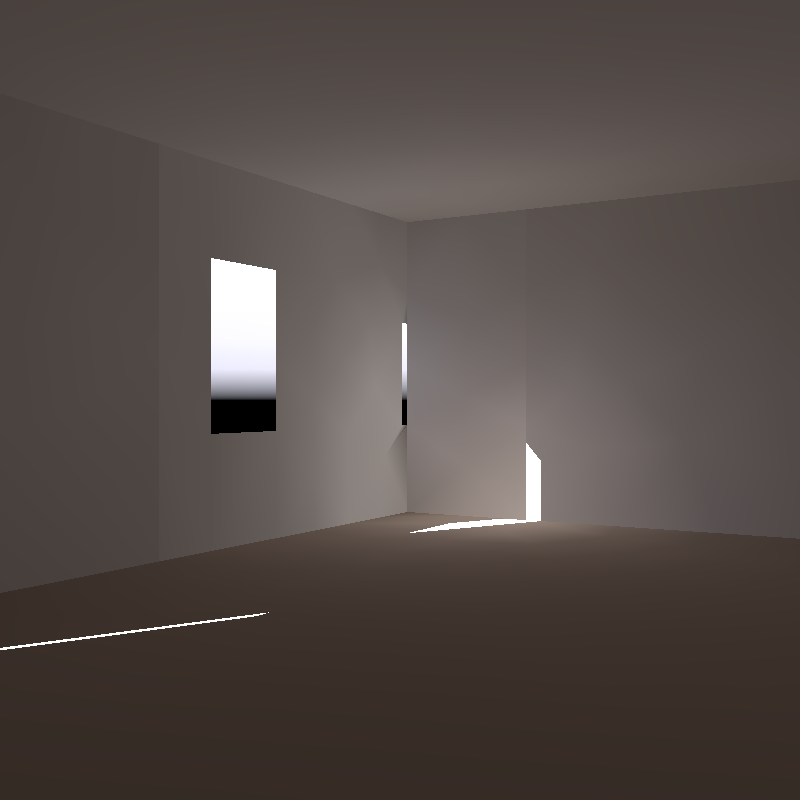
\includegraphics[width=0.158\textwidth]{../gi2012_userstudy/images/renderings/renovations/user_046_camera_chris_march.png}
\\
\begin{sideways}~~Camera 2\end{sideways}&
  \includegraphics[width=0.158\textwidth]{../gi2012_userstudy/images/renderings/renovations/063_camera_dark_march_crop.png}
  \includegraphics[width=0.158\textwidth]{../gi2012_userstudy/images/renderings/renovations/050_camera_dark_march_crop.png}
  \includegraphics[width=0.158\textwidth]{../gi2012_userstudy/images/renderings/no_renovations/070_camera_dark_march_crop.png}
  \includegraphics[width=0.158\textwidth]{../gi2012_userstudy/images/renderings/renovations/098_camera_dark_march_crop.png}
  \includegraphics[width=0.158\textwidth]{../gi2012_userstudy/images/renderings/no_renovations/user_085_camera_dark_march_crop.png}
  \includegraphics[width=0.158\textwidth]{../gi2012_userstudy/images/renderings/renovations/user_046_camera_dark_march_crop.png}
\end{tabular}
\\ 

  \vspace{-4.8in}
  %
  \hspace{.5in}
\begin{minipage}{0.158\textwidth}~{\color{white}{\bf N1}}\end{minipage} 
\begin{minipage}{0.158\textwidth}~{\color{white}{\bf N2}}\end{minipage}
\begin{minipage}{0.158\textwidth}~{\color{white}{\bf N3}}\end{minipage}
\begin{minipage}{0.158\textwidth}~{\color{white}{\bf N4}}\end{minipage}
\begin{minipage}{0.158\textwidth}~{\color{white}{\bf N5}}\end{minipage} 
\begin{minipage}{0.158\textwidth}~{\color{white}{\bf N6}}\end{minipage} \\
\vspace{3.7in}

\ \vspace{0.0in} 
\\ 
{\em Simulation results for the original room geometry
  constructed by the study participants.  The ground-truth model was
  constructed with the same tangible interface using the true room
  dimensions.  All models are constructed using the same floor, wall,
  and ceiling materials.  All renderings in this figure are March 21st
  at 8:30am.  The desks in the southwest corner of the room (1st and
  3rd rows) experiences glare at this time.  The east side of the room
  (2nd and 4th rows) is quite dark all year, especially in the
  mornings.  }\\\\
\begin{comment}
  \begin{tabular}{lc}
\begin{sideways}~~September 21\end{sideways}&
  \includegraphics[width=0.158\textwidth]{../gi2012_userstudy/images/renderings/renovations/065_camera_chris_march.png}
  \includegraphics[width=0.158\textwidth]{../gi2012_userstudy/images/renderings/renovations/065_camera_chris_march_mod.png}
  \includegraphics[width=0.158\textwidth]{../gi2012_userstudy/images/renderings/renovations/031_camera_chris_march.png}
  \includegraphics[width=0.158\textwidth]{../gi2012_userstudy/images/renderings/renovations/031_camera_chris_march_mod.png}
  \includegraphics[width=0.158\textwidth]{../gi2012_userstudy/images/renderings/renovations/063_camera_chris_march.png}
  \includegraphics[width=0.158\textwidth]{../gi2012_userstudy/images/renderings/renovations/063-2_camera_chris_march_mod.png}
\\
\begin{sideways}~~September 21\end{sideways}&
  \includegraphics[width=0.158\textwidth]{../gi2012_userstudy/images/renderings/renovations/065_camera_chris_march.png}
  \includegraphics[width=0.158\textwidth]{../gi2012_userstudy/images/renderings/renovations/065_camera_chris_march_mod.png}
  \includegraphics[width=0.158\textwidth]{../gi2012_userstudy/images/renderings/renovations/063_camera_dark_december_crop.png}
  \includegraphics[width=0.158\textwidth]{../gi2012_userstudy/images/renderings/renovations/031_camera_dark_december_mod_crop.png}
  \includegraphics[width=0.158\textwidth]{../gi2012_userstudy/images/renderings/renovations/063_camera_dark_december_crop.png}
  \includegraphics[width=0.158\textwidth]{../gi2012_userstudy/images/renderings/renovations/063-2_camera_dark_december_mod_crop.png}
\end{tabular}
\\ 
\ \vspace{0.0in} 
\\ 
{\em To address the general gloominess of the room, participants
  suggest adding more, taller, and/or wider windows on the southern
  wall.  Some participants also
  removed the existing interior wall/partition that was deemed to be
  an obstruction to daylighting.  While these modifications did
  brighten the room considerably, it will also increase the glare
  problems for those working at desks in the path of the light.
  Renderings in the top row are March 21st at 8:30am and the bottom
  row shows December 21st at 3pm. }\\

\vspace*{0.5in}
\end{comment}
\begin{tabular}{lc}
%\vspace{.5in}
\begin{sideways}~~~~~~~Camera 1\end{sideways}&
  \includegraphics[width=0.158\textwidth]{../gi2012_userstudy/images/renderings/renovations/065_camera_chris_march.png}
  \includegraphics[width=0.158\textwidth]{../gi2012_userstudy/images/renderings/renovations/065_camera_chris_march_mod.png}
%  \includegraphics[width=0.158\textwidth]{../gi2012_userstudy/images/renderings/renovations/050_camera_chris_march.png}
%  \includegraphics[width=0.158\textwidth]{../gi2012_userstudy/images/renderings/renovations/050_camera_chris_march_mod.png}
  \includegraphics[width=0.158\textwidth]{../gi2012_userstudy/images/renderings/renovations/user_046_camera_chris_march.png}
  \includegraphics[width=0.158\textwidth]{../gi2012_userstudy/images/renderings/renovations/user_046_camera_chris_march_mod.png}
  \includegraphics[width=0.158\textwidth]{../gi2012_userstudy/images/renderings/renovations/042_camera_chris_december}
  \includegraphics[width=0.158\textwidth]{../gi2012_userstudy/images/renderings/renovations/042_camera_chris_december_mod}
  \\
%\\
%\vspace{-1.5in}
\begin{sideways}~~Camera 2\end{sideways}&
  \includegraphics[width=0.158\textwidth]{../gi2012_userstudy/images/renderings/renovations/065_camera_dark_march_crop.png}
  \includegraphics[width=0.158\textwidth]{../gi2012_userstudy/images/renderings/renovations/065_camera_dark_march_mod_crop.png}
%  \includegraphics[width=0.158\textwidth]{../gi2012_userstudy/images/renderings/renovations/050_camera_dark_december_crop.png}
%  \includegraphics[width=0.158\textwidth]{../gi2012_userstudy/images/renderings/renovations/050_camera_dark_december_mod_crop.png}
  \includegraphics[width=0.158\textwidth]{../gi2012_userstudy/images/renderings/renovations/user_046_camera_dark_march_crop.png}
  \includegraphics[width=0.158\textwidth]{../gi2012_userstudy/images/renderings/renovations/user_046_camera_dark_march_mod_crop.png}
  \includegraphics[width=0.158\textwidth]{../gi2012_userstudy/images/renderings/renovations/042_camera_dark_december_crop.png}
  \includegraphics[width=0.158\textwidth]{../gi2012_userstudy/images/renderings/renovations/042_camera_dark_december_mod_crop.png}


\end{tabular}

\vspace{-4.6in}
\hspace{.5in}
\begin{minipage}{0.158\textwidth}~{\color{white}{\bf A1 original}}\end{minipage} 
\begin{minipage}{0.158\textwidth}~{\color{white}{\bf A1 renovation}}\end{minipage}
%
\begin{minipage}{0.158\textwidth}~{\color{white}{\bf N6 original}}\end{minipage} 
\begin{minipage}{0.158\textwidth}~{\color{white}{\bf N6 renovation}}\end{minipage} 
%\hfill
\begin{minipage}{0.158\textwidth}~{\color{white}{\bf A3 original}}\end{minipage} 
\begin{minipage}{0.158\textwidth}~{\color{white}{\bf A3 renovation}}\end{minipage}
%
\vspace{4.1in}
{\em \\To address the general gloominess of the room, participants
  suggest adding more, taller, and/or wider windows on the southern
  wall.  Some participants also
  removed the existing interior wall/partition that was deemed to be
  an obstruction to daylighting.  While these modifications did
  brighten the room considerably, it will also increase the glare
  problems for those working at desks in the path of the light.
  Only a few of the participants suggested renovations that
  attempt to mitigate the glare problems in the space through new
  geometry in the model.  These proposals involve the addition of
  partitions that diffusely redirect the harsh direct southern light
  for more usable daylighting.
}



\label{FIGURE_results_changing_time}
\vspace{-6in}
\end{minipage}
%%%%%%%%%%%%%%%%%%%%%%%%%%%%%%%%%%%%%%%%%%%%%%%%%%%%%%%%%%%%%%%%%%%%%%%%%%%%%%%%%%%%%%%
%%%%%%%%%%%%%%%%%%%%%%%%%%%%%%%%%%%%%%%%%%%%%%%%%%%%%%%%%%%%%%%%%%%%%%%%%%%%%%%%%%%%%%%


\end{document}

